%%%%%%%%%%%%%%%%%%CHAPTER BREAK%%%%%%%%%%%%%%%%%%%%%%%%%%%%%%%%%%%%%%%%%%%%%%%%%%%%%%%%%%%%%%%%%%%%%%%%
\chapter{Problem Settings}

As the society of IOT (internet of things) develops, many learning platforms shifted from offline classrooms such as schools or tutoring centers to online educational platforms such as Coursera \cite{Coursera}, Udemy \cite{Udemy}, and Teachable \cite{Teachable}. Second language learning is a major part of education curriculum. The process of natural language learning can be mainly split into four parts, listening, speaking, reading, and writing. Among these four topics, reading is often recognized as the most important aspect \cite{chi2007designing}. In the traditional settings such as in school or one-to-many tutoring, same second language reading materials are given to all students despite that every student's profile including learning habit, current language skill level, and etc is very different. 

To solve this problem, many researchers proposed the idea called personalized article recommendation \cite{Hsu2008, Liu2009, Hsu2013, Tan1998, Kuo2014}. Most of the existing researches were carried out in the traditional settings which are inside the school classroom \cite{Hsu2008, Hsu2013, Kuo2014}. These studies mainly focus on how to recommend articles to students at school and their methods are restricted in this traditional specific settings. Majority of the existing work proposes to use complicated pre-tests to obtain the user profile and to have language experts to label the reading in the databases \cite{Hwang2010}. These kinds of actions are only allowed in the traditional settings due to the small user scale. However, when it comes to personalized recommendations based upon user language level in a large-scale online user application, many methods proposed in the existing studies will not be applicable.

In most of the online news or article applications, recommendation system is a necessity to filter out relative information to specific users among the overwhelming articles that exist on the internet. These traditional reading recommendation systems usually focus merely on recommending readings that suit user's interest or based upon the current trend such as popularity and big events. However, for second language learners using these traditional online article application, the title of the reading that is recommended to these learners could be very attractive, but the body of the reading could be linguistically too difficult for these learners to understand, which causes them to dislike the recommendation and stop reading. So a simple question to be answered is that: 
\subsubsection{Are the current online article recommendation systems suitable to users reading articles in their second language?}
\vspace{10pt}

In this study, instead of following the existing studies which focus on solving the personalized recommendation problem in the traditional settings, we decided to look at the problem from a different perspective. Because of development of IOT, many education systems have been slowly shifted from offline to online \cite{Coursera, Udemy, Teachable}. Newsela \cite{Newsela} is an online article application that is specifically designed for English learners. There exist many more online reading applications for language learning just like Newsela. In this study, we decided to carry out our research in an online large scaled user application problem settings and we sought a method that is suitable to the proposed problem settings unlike any of the existing methods.

%%%%%%%%%%%%%%%%%%CHAPTER BREAK%%%%%%%%%%%%%%%%%%%%%%%%%%%%%%%%%%%%%%%%%%%%%%%%%%%%%%%%%%%%%%%%%%%%%%%%

\chapter{Literature Review}

\section{Overview}

There are numberless applications that assist learner studying natural languages. Most of the applications focus on helping individuals study a second language such as English and Japanese using their first language. Each application uses different technologies to assist language learning. Shinohara did research on using audiovisual training to correct Japanese English pronunciation \cite{Shinohara2016} and Luo did research on using dubbing practice to train English learners' speaking skill \cite{Luo2016}. However, when it comes to reading recommendations based on user language level, there only exists a very limited amount of previous studies. To be able to recommend articles based upon user language level, the system needs to be capable of finding out the distance between the article and the user, more specifically how difficult the article is in correspondence to each user's language level. One way of finding out the distance between the user and the article is to determine the article readability and user language level separately. The other is to find out the distance directly using measures such as relative difficulty \cite{Carver1994}. The following of this chapter is organized as follows:
\begin{enumerate}
  \item Background information and terminology will be introduced in section Article Readability, User Language Level, Relative Difficulty, and Computerized annotations.
  \item Studies that have researched on a similar topic as the one proposed in this thesis are provided in section Existing Personalized Recommendation.
  \item Finally, the limitations of the existing work will be explained in section Limitation of the existing methods
\end{enumerate}

\section{Article readability}

Reading readability (also called difficulty) is often used to estimate the linguistic complexity of texts or sentences, so that language learners can choose proper learning materials. One of the most fundamental obstacles in natural language processing is how to assess reading readability. Heilman \cite{Heilman2007} described reading difficulty as a function that is capable of mapping a reading material to a numerical value corresponding to a difficulty or grade level. In most of the studies, researchers extracted series of lexical and grammatical features (such as text length, word frequency, and grammatical complexity) from a document acting as the inputs of this function, and it outputs a numerical value which describes the difficulty of the document.

The issue of reading difficulty has been studied by many researchers who have applied various lexical and grammatical features in statistic models to analyze this problem. The very early studies such as the Dale-Chall readability formula \cite{DaleChall1995,DaleChall1948}, the Flesch-Kincaid measures \cite{Kincaid1975}, and the Lexile Framework \cite{Lexile1996} only used simple lexical and grammatical features as input and developed a regression model to predict the reading difficulty levels. By adopting more complicated features, Schwarm and Ostendorf \cite{Ostendorf2005} demonstrated that their model can significantly increase the performance of readability prediction. While all the above studies are designed for native language readers, Huang \cite{Huang2011} proposed a system that adopts features specifically for second language learner in Taiwan, which outperforms previous models in the situation of non-native speakers learning English. Most recent researches started to adopt machine learning models to measure the reading difficult, such as Ildiko and Sowmya's work \cite{ElenaSowmya}.

Flesch-Kincaid score and Lexile score are the two primary metrics used in this study to determine the articles' readability. Equation (\ref{eq:flesch_kincaid}) shows the calculation of Flesch reading-ease score (FRES).
\begin{equation}\label{eq:flesch_kincaid}
  FRES = 206.835 - 1.015\frac{total \, words}{total \, sentences} - 84.6\frac{total \, syllables}{total \, words}
\end{equation}
Flesch reading-ease score can be interpreted as shown in the Table \ref{table:flesch_kincaid} below \cite{flesch1979write}. In general, a lower flesch reading-ease score indicates a higher readability of an article.
\begin{table}[btp]
 \caption{\label{table:flesch_kincaid} The interpretation of the FRES}
 \begin{center}
  \begin{tabular}{ccc}
   \hline
   Score & School level & Notes \\
   \hline
   100.00-90.00 & 5th grade & Very easy to read. \\
   90.00-80.00 & 6th grade & Easy to read. \\
   80.00-70.00 & 7th grade & Fairly easy to read. \\
   70.00-60.00 & 8th \& 9th grade & Plain English. \\
   60.00-50.00 & 10th to 12th grade & Fairly difficult to read. \\
   50.00-30.00 & college & 	Difficult to read. \\
   30.00-0.00 & college graduate & Very difficult to read. \\
   \hline
  \end{tabular} 
 \end{center}
\end{table}

Lexile Framework on the other hand is not an open-sourced program. The Lexile Analyzer \cite{LexileAnalyzer} is used to find the Lexile score of all the readings in the database. In general, the Lexile score increases as the reading's readability increases.

\section{User language level}

User language level is a measurement used to define the language fluency of users. Traditionally, user language level is measured through numerous tests such as TOEFL, TOEIC for English language level, and N1 for Japanese language level. However, traditional means of measuring user language level is certainly not applicable to user applications since it will require all the users in the application to take certain tests before they can actually use the application. Numerous researches have devoted to determining user language level through simple tasks. Kise \cite{Yoshimura2015} proposed a method of using the eye tracking devices to analyze user's eye movement while doing readings to predict user's language level. Hwang \cite{Hwang2008, Hwang2010} designed a search engine system that tracks students' search keyword to build a knowledge base of each student in order to measure the user language level. Kuo \cite{Kuo2014} conducted a research which takes user's own writings as input and extracts lexical and grammatical features from these writings to measure the user language level.

\section{Relative difficulty}

\begin{figure}[tbp]
 \begin{center}
  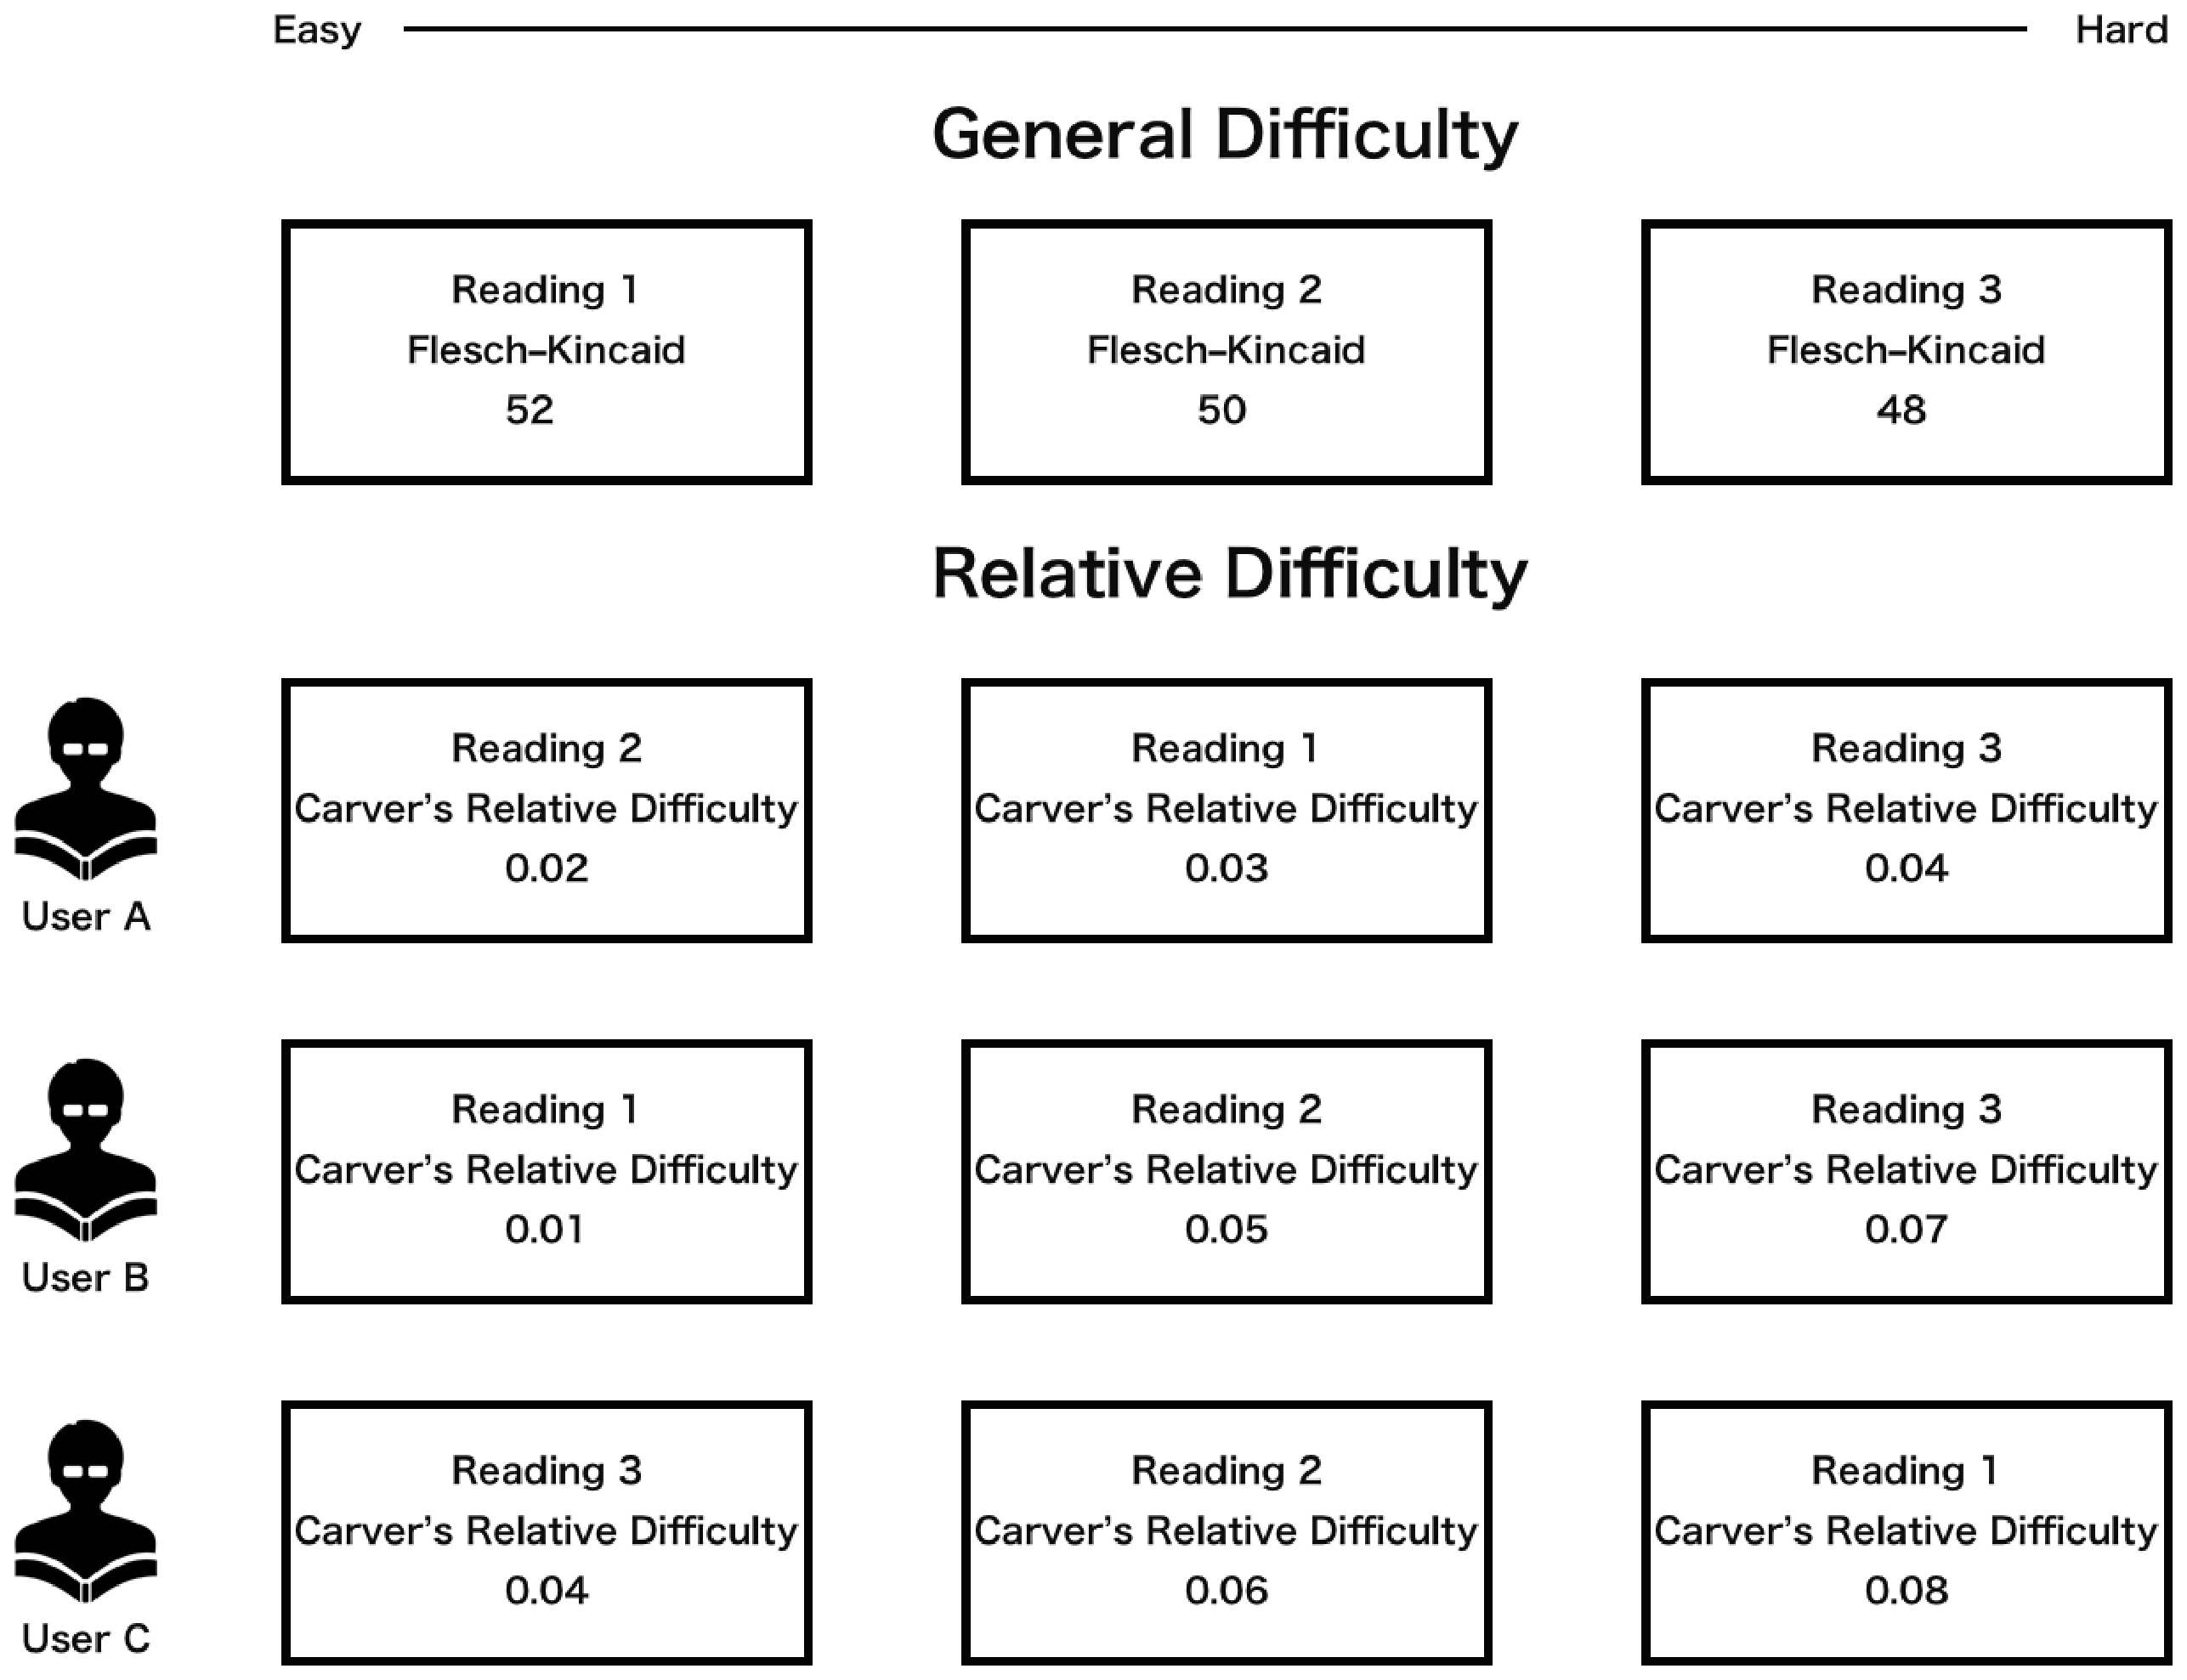
\includegraphics[width=120mm]{relative_vs_general.eps}
 \end{center}
 \caption{\label{figure:relative_vs_general} Illustration of the relative difficulty and the general difficulty}
\end{figure}

The relative difficulty is a terminology that is used throughout this paper. If we call the reading difficulty measurements such as Dale-Chall readability formula \cite{DaleChall1995, DaleChall1948}, the Flesch-Kincaid measures \cite{Kincaid1975}, and the Lexile Framework \cite{Lexile1996} as general difficulty meaning that all these measures provide an average hardness of the reading towards an average linguistically skilled individual, relative difficulty is the measure that illustrates the difficulty of a specific reading corresponding to a specific user \cite{Carver1994}.

Because every user's language skill is different and everyone has a different knowledge base (such as knowing specific terminologies in the medical field), one specific reading's readability should be different for each user. For instance, a user with a medical background can easily understand a medical-related article. But It will be much harder for a non-medical background individual to understand the same article. But this difficulty difference between these two individuals will not be shown if we only look at the readability measures of the reading.

Carver \cite{Carver1994} also approves the idea of relative difficulty and proposed a definition of relative difficulty which is measured by the percentage of unknown words that the user has towards one specific reading. This study adopts Carver's definition of relative difficulty as the measurement of the distance between a specific user to a specific reading. Carver's definition of relative difficulty will be used as the basis for the recommendation model that we will propose later in this paper. Equation (\ref{eq:carver_relative_difficulty}) shows Carver's definition of Relative Difficulty.

\begin{equation}\label{eq:carver_relative_difficulty}
   Carver's \, Relative \, Difficulty = \frac{Number \, of \, unknown \, vocabulary}{Number \, of \, total \, unique \,vocabulary \, in \, the \, reading}
\end{equation}

Figure~\ref{figure:relative_vs_general} is an illustration of the difference between the relative difficulty and the general difficulty. The general difficulty of a reading is always fixed if the same readability measure is used, because all the features that used to determine the general difficulty is within the content of the reading itself. Therefore, the ranking of the articles based on the general difficulty is always the same for every user. On the other hand, the relative difficulty takes in features from both the reading and the user as shown in Equation (\ref{eq:carver_relative_difficulty}), which leads to a more personalized measure of the difficulty of each reading. Hence, the ranking by relative difficulty changes based on each user language level. 

\begin{figure}[tbp]
 \begin{center}
  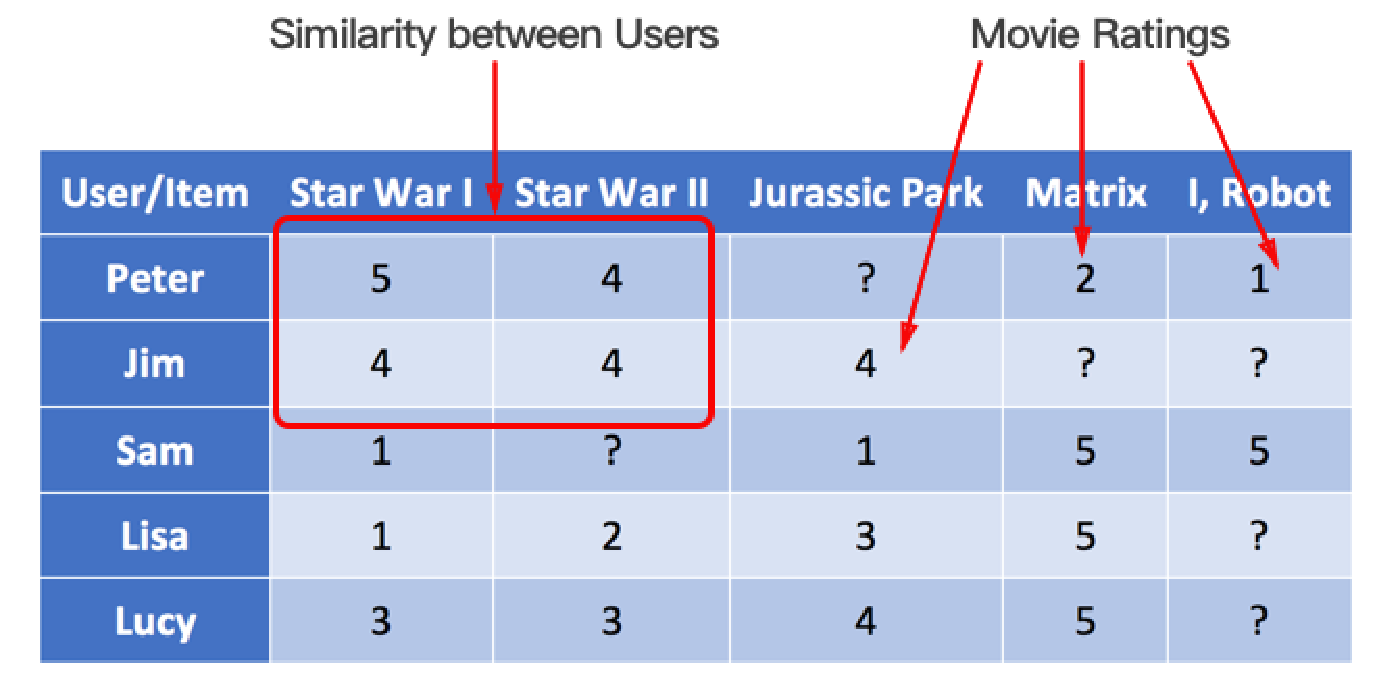
\includegraphics[width=100mm]{movie_matrix.eps}
 \end{center}
 \caption{\label{figure:rating_matrix} A typical movie rating recommedation matrix}
\end{figure}

\section{Collaborative filtering}

\begin{figure}[tbp]
 \begin{center}
  \includegraphics[width=90mm]{basic_idea_CF.eps}
 \end{center}
 \caption{\label{figure:collabrative_filering_explain} The basic idea of collabrative filtering}
\end{figure}

Collaborative filtering is a method often used by recommendation systems \cite{Ricci2011}. It is a process of data filtering to find specific information, patterns, or similarities using techniques involving collaboration among multiple users. Typical collaborative filtering system will construct a 2-d recommendation matrix based upon all users' profiles. Figure~\ref{figure:rating_matrix} is an example of a rating recommendation matrix, where each column indicates a different user and each row indicates a different item. So the cell at column A and row W means user A gives item W a rating of 4. Each column in the matrix is a user profile vector whereas each row in the matrix is an item profile vector. By using similarity measures such as Cosine similarity or Euclidean distance [40] between these vectors, collaborative filtering is capable of finding similar users and predict the ratings of unknown items. 
Formula (\ref{eq:cosine_similarity}) shows the equation of consine similarity whereas Formula (\ref{eq:euclidean}) shows the equation of Euclidean distance.
\begin{equation}\label{eq:cosine_similarity}
  Cosine \, Similarity = cos(x, y) = \frac{x \cdot y}{||x|| \cdot ||y||}
\end{equation}

\begin{equation}\label{eq:euclidean}
  Euclidean \, Distance = \sqrt{\sum_{i=1}^n (x_i-y_i)^2}
\end{equation}

\section{Computerized annotations}

The advancement of network and computer technologies encourages users nowadays to carry out reading activities on the web or in electronic form \cite{Huang2009}. Many webs or electronic text readers provide users with annotation functionalities, such as notes annotation (such as Adobe's pdf expert) \cite{Makany2009} or translation annotation (such as amazon's kindle) \cite{Hsu2013}. Scholars have found that using annotation while reading can reduce the cognitive load of students, which can ease the understanding of the reading material \cite{Dror2008}.

Figure~\ref{figure:kindle} shows the interface of Amazon Kindle's translation annotation module.
\begin{figure}[tbp]
 \begin{center}
  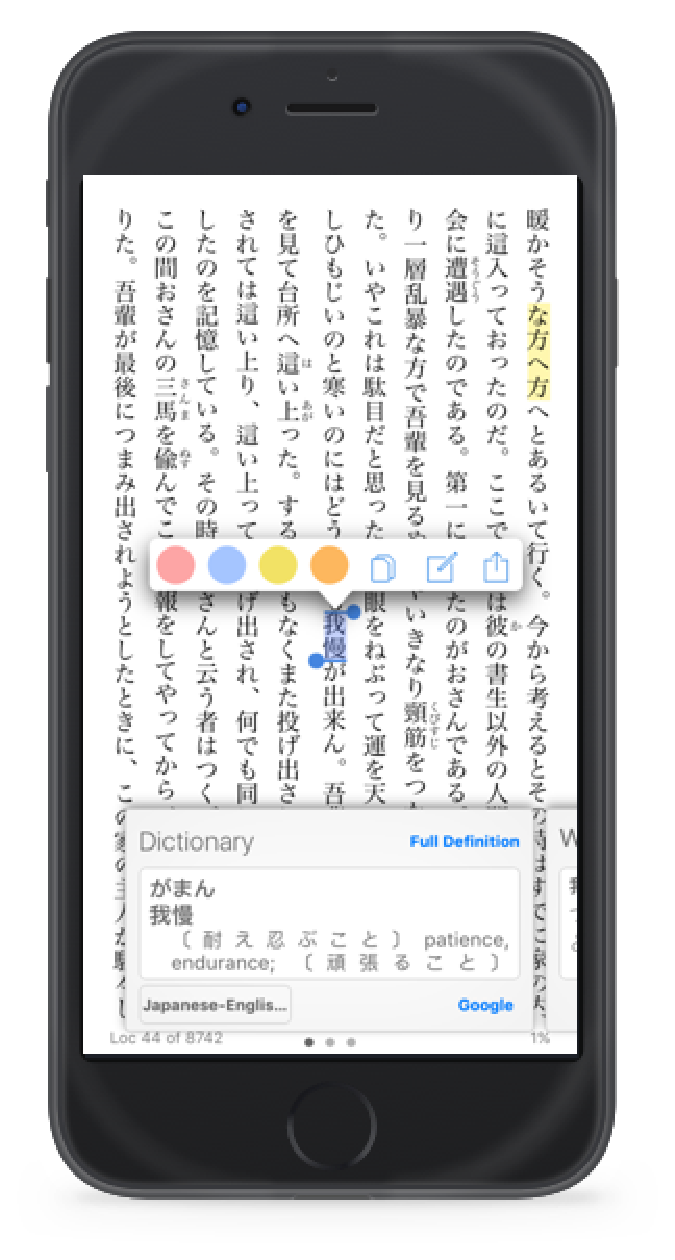
\includegraphics[width=50mm]{kindle_annotation.eps}
 \end{center}
 \caption{\label{figure:kindle} The interface of translation annotation module in Kindle}
\end{figure}

Several studies suggested that students who make annotations while reading tend to outperform those who do not take any action while doing reading \cite{Brown1978}. Quade \cite{Quade1996} conducted a study that demonstrated that students tend to achieve the better learning outcomes while using computers to take notes than using pen and paper. This study installs a translation annotation module into the recommendation system that simulates the translation annotation process of second language learner when running into unknown vocabulary while doing readings. Users can simply touch on the word that they are not familiar with, the system will provide translations to their native language.

\section{Existing personalized recommendation system}

Most of the online learning applications provide same teaching materials to all users, however, towards different users, the same materials can be too easy or too hard \cite{Tang2005}. To solve this issue, researchers have developed various recommendation systems or adaptive learning systems that are capable of providing personalized learning materials to individual students by analyzing their profiles or learning portfolios \cite{Hsu2013, Kuo2014}. For example, CAMLES \cite{Nguyen2010} is a personalized context-aware mobile learning application for supporting students to learn English as a foreign language in order to prepare for TOEFL test. The system provides adaptive content for different learners based upon individual context. In their model, the individual context includes many parameters such as location (places that the study takes place, i.e. restaurant), time (what time of the day the study takes place), manner (i.e., concentration, interest level) as well as learner's knowledge. By analyzing the parameters above combining with the answers to the questions at the end of each study, the system adaptively pushes appropriate material to the users. 

The University of Rijeka in Croatia is also currently developing an adaptive e-learning system for language learning on a web platform. \cite{jugo2016increasing} As shown in their proposed adaptive language e-learning system, they developed a system that constantly evaluates learners' skill and providing suitable educational content based upon individual language competence. 

In the meantime, several learning systems specifically designed for language learning with recommendation mechanisms have been developed. For example, Kuo \cite{Kuo2014} has adopted the idea of Input hypothesis \cite{Krashen1987} stating that when a learner is at stage I, then acquisition occurs when a learner is exposed to comprehensible input that belongs to the level I + 1. In his research, he extracted features such as vocabulary difficulty and sentence length from each article and classify them into three category based upon text similarity using the above features: Level I (The level that learner currently belongs to), Level I + 1 (The level that learner needs to read at to acquire knowledge), and Level I + 2 (The level that is too difficult for the user). To determine each user's language level I, the system takes user's writings as input and uses machine learning method kNN and Naive Bayes to predict the difficulty level of the readings. 

\section{Limitation of the existing methods}
There are many limitations to the existing methods:

\subsubsection{Not applicable to a large-scale user application}
\vspace{10pt}
Most of the existing researches were carried out in the traditional settings which are inside the school classroom from elementary school class to college class. All the methods share a limitation which is restricted to the small-scale user environment. Majority of the existing work proposes to use complicated pre-tests to obtain the user profile and to have language experts to label the reading in the databases \cite{Kuo2014, Hwang2010}. These heavy prerequisites will only work in school because students are very obedient to teachers' request. However, if the same method is applied to an online large scaled user application, the heavy prerequisites of the existing method will stop many interested users from trying the application due to the bad user experience. Only very few users are willing to take on heavy pre-test before they can use the application. 

\subsubsection{Not capable of updating user profile change later on}
\vspace{10pt}
Existing work only collects user's profile once at the beginning of their experiments by asking users to manually input their information through pre-test or similar. The user profile in their system never changes after the first collection. This means that the system is not capable of adapting to user's change in language level and recommend items according to these changes. However, users language level does change a lot especially for second language learners who try to absorb as much knowledge as they can every day. Most of the existing methods lack the ability to automatically create and update user's profile and adapt to user's change in language ability later on.

\subsubsection{No accurate metric to determine the distance between a user and a reading}
\vspace{10pt}
Most of the existing work tried to find out both user language level and articles readability to match a user with specific language level to an article with specific difficulty. However, regular way of determining the difficulty of the reading only depends on the features of the article itself. It ignores the feature of the user. A reading of difficulty 10 could be as easy as 1 for a native speaker while a reading of difficulty 1 could be as hard as 10 for a beginner. As Carver suggested, there is a relative difficulty between one specific reading and one specific user. Most of the existing methods haven't used any metric similar to the relative difficulty to accurately define the distance between a reading and a user. 

%%%%%%%%%%%%%%%%%%CHAPTER BREAK%%%%%%%%%%%%%%%%%%%%%%%%%%%%%%%%%%%%%%%%%%%%%%%%%%%%%%%%%%%%%%%%%%%%%%%%

\chapter{Recommendation Beased on Weighed Relative Difficulty}

\section{Overview}

In this study, a responsive web application, Adaptive Learner, was developed in this research for both data collection and experimental purpose. Adaptive Learner includes an estimator that predicts the relative difficulty of a reading for a user, a reading recommendation system that will suggest readings to each user based upon the prediction of relative difficulty from the estimator, and a translation annotation module that allows users to translate any unknown words or phrase into their native language by simply selecting these words or phrases.

% traditional recommender
In a traditional article recommendation system, constructing an accurate profile of each user's interests is essential for the recommendation systems to be successful. \cite{liu2010personalized} There exist many means of obtaining an accurate user profile. One of the most typical ways of acquiring user profile is asking users to manually create their profile before they start using the application and later on ask them to update their profile if their interest changes. According to Liu \cite{liu2010personalized}, this kind of approach places an extra burden on users, something very few are willing to take on. Instead, many systems take the approach of constructing the user profiles automatically from users' interaction with the system. These interactions include elements such as followings:
\subsubsection{Tracking user's clicking}
\vspace{10pt}
Through tracking all articles that user has clicked on, it becomes easy to distinguish what kind of category that this user is interested in.
\subsubsection{The length of time that a user has spent on a reading}
\vspace{10pt}
By tracking the time that a user has spent on a reading, it can be easily determined whether a user has finished the reading or not. If a user exits from an article very fast, the system can read this action as a misclick and update the user profile.
\subsubsection{Whether a user has commented on an article}
\vspace{10pt}
Commenting action requires a user to take time and efforts which usually indicates that user is paying extra attention to this article.

Tracking users' interaction with the system and automatically create and update user's profile has become the default requirements in most of the large-scale user applications today. Automatically updating user's profile also allows the system to be able to adapt quickly to sudden changes in user's interest. Good user experience is an essential requirement for a user-oriented application to success. Anything that gives extra burden such as manually creates a user profile to the users will not work in an online large-scale user application. Because this study focus specifically on dealing with personalized article recommendation based on user language level, it is necessary for us to find a way to automatically create and update users' profile as well as detect users' improvement or decline in their language level. 

To avoid putting extra burdens on the users to create and update user profile through pre-test as it was done in most of the previous studies, in the proposed system, a translation annotation module is integrated to achieve the automation of creating and updating users' language level profile as it is being done in most of the online recommenders today. The translation annotation module allows users to select any unknown words or phrases to see its translation in their native language. The translation annotation module current supports translating English to Chinese and English to Japanese. When users read articles on the proposed the system and use the translation annotation module to find meanings for unknown words, the system can construct a user profile of each user's known and unknown words. The next question is how to utilize this user profile information to recommend personalized articles to the users based on their language level.

To utilize users' unknown clickings from the translation annotation module, Carver's Relative Difficulty is adopted. Carver states that there is a relative difficulty between one specific reading to one specific user, and one way of measuring the relative difficulty is through the percentage of unknown words that a user has towards a specific reading. By utilizing the users' unknown clickings data, Carver's relative difficulty can be easily calculated. And by calculating the relative difficulty of each reading towards each user, the system can obtain the distances between each user and each reading.

Carver's relative difficulty is used as the foundation for the recommendation system proposed in this study. Because the relative difficulty illustrates the distance between a reading and a user, knowing the relative difficulty means accurately understanding how hard a reading is for a specific user. And the recommender system can simply use the relative difficulty of a reading towards a user to recommend items that suit user's current language level. Hence, we believe that it is critical to predict the relative difficulty of each reading towards each user in order to make appropriate articles to users in our system. However, through the experiment phase, we realized that unlike the experiment that Carver has conducted in his research where every student intentionally circles out every unknown word in the reading, in the proposed system, there exist many human errors such as misclicking and unknown words that weren't clicked by the users. In Carver's definition of relative difficulty, every unknown word is weighted equally. However, this seems to be flawed in our problem settings. To deal with this issue, we proposed a weighted relative difficulty derived from Carver's definition. The proposed weighted relative difficulty uses frequency of the words as standard to apply a weight on every unknown word that user has clicked through the translation annotation module. By doing so, a word with a higher frequency such as ‘the' and ‘you' will weigh less to reduce the effect of misclicking on these words whereas a word with a lower frequency will weigh higher to increase its importance in calculating relative difficulty. 

To predict the relative difficulty, an estimator for relative difficulty is proposed in this study. Both definitions of relative difficulty (Carver's and ours) are passed in as features to the various estimators to find out which relative difficulty measure is better at determining the distance between a reading and a user. One type of estimator algorithms that was attempted in this study is to call collaborative filtering \cite{Ricci2011}, which is one of the most popular recommendation methods. 

Collaborative filtering is a process of data filtering to find specific information, patterns, or similarities using techniques involving collaboration among multiple users. Typical collaborative filtering system will construct a 2-d recommendation matrix based upon all users' profiles. In a simple traditional reading recommendation system, the data used in the 2-d recommendation matrix could be 1 and 0 where 1 stands for a user has read an article and 0 stands for a user has not read an article. So if both user A and user B have read similar types of articles, then if user A has read an article that user B hasn't read, since these two users are so similar, the traditional recommender will recommend this item to user B.

In this study, the data passed into the 2-d recommendation matrix is the relative difficulty. Two different 2-d recommendation matrices were constructed using both Carver's definition of relative difficulty and ours. 8 different collaborative filtering algorithms were tested with the collected datasets. Another type of estimator that is also tested in this study is the linear regression estimator. Due to the continuity feature of relative difficulty which is shown in the collected dataset, linear regression estimator is also attempted and compared with the collaborative filtering based methods. 

The personalized recommendation system takes the estimator's prediction of a user's relative difficulty of each reading as input and ranks articles with relative difficulty. The recommendation system suggests articles with lower relative difficulty to each user to ensure that the content of the article is understandable. In the proposed system, each article will be labeled with relative difficulty which is estimated specifically for each user. Learners using the proposed system can also challenge articles with higher relative difficulty.

Figure~\ref{figure:system_design_schmatic} shows the design schematics of the proposed system, which consists of five major module including:
\begin{enumerate}
  \item a database where all the readings, user info, and tracking data were stored,
  \vspace{10pt}
  \item a server where all API calls such as user login were handled,
  \vspace{10pt}
  \item a responsive web interface with the translation annotation module where users read all the articles at,
  \vspace{10pt}
  \item a relative difficulty estimator where each user's relative difficulty of each unread article is predicted,
  \vspace{10pt}
  \item and the reading recommendation system where appropriate article recommendations are suggested to each user based on the relative difficulty estimator.
  \vspace{10pt}
\end{enumerate}

Many technologies are used in this study including:
\begin{enumerate}
  \item MongoDB for the database, 
  \vspace{10pt}
  \item Meteor Framework for backend development,
  \vspace{10pt}
  \item React and Redux for frontend responsive web application,
  \vspace{10pt}
  \item NTLK toolkit for lexical manipulation of the texts,
  \vspace{10pt}
  \item Surprise package for developing the proposed reading recommendation system,
  \vspace{10pt}
  \item And Scikit-learn for evaluation of the proposed methods
  \vspace{10pt}
\end{enumerate}

\begin{figure}[tbp]
 \begin{center}
  \includegraphics[width=120mm]{system_design.eps}
 \end{center}
 \caption{\label{figure:system_design_schmatic} The overall system design schmatic}
\end{figure}

\section{Translation annotation module}

Csikszentmihalyi \cite{Csikszentmihalyi2002, Csikszentmihalyi1997, Csikszentmihalyi1975} proposed a concept called flow, which is a state that people will enter while performing any activity. A person is most likely to enter a flow state while wholeheartedly concentrating on a task or activity for intrinsic purposes. Krashen also proposed similar idea regarding language learning indicating that language learners are more likely to acquire knowledge if he/she is in the right state of mind. However, flow state can be easily broke out of due to reasons such as boredom or anxiety. It is particularly hard to be in a flow state if a person is reading materials that are much more difficult than his/her language level. One of the reasons that a hard reading material may break user's flow state is unknown vocabulary. A very typical action that a language learner does when he/she runs into unknown words is simply using a dictionary or translation application to find out the meaning of the word. However, this translation action will take user's eyes away from the reading, which ends the flow state. And readings with a lot of unknown words will cause this translation action to repeat many times which may lead to user's annoyance and lose interest in the articles. 

Carver \cite{Carver1994} proposed a formula for measuring relative difficulty between a specific user and a specific reading. The formula requires the amount of unknown vocabulary that a user has towards a reading and the amount of total unique words that a reading contains. During Carver's experiment, to find out the relative difficulty, he simply conducted an experiment that asked all users to circle out the words that they are not familiar with in the reading and counted these circles manually. In our research, to calculate the relative difficulty of each user toward each reading, we will have to collect the number of unknown words that each user has towards each reading. 

To solve the two problems above, a translation annotation module is added to our system. Users can click on any unknown words, our translation annotation module will provide dictionary meanings in user's native language. Users can also select multiple words or sentences to see a machine-translated meaning of the selected texts. The translation module currently supports translations from English to Chinese and English to Japanese. By using the translation annotation module, users no longer need to look up unknown vocabulary on another device or an actual dictionary. By stopping users from looking away from the reading materials to look up unknown words' meanings, it helps users stay focused on the material and stay in the flow state. On the other hand, by collecting the unknown words that user has selected, we can find out the amount of the unknown words that a user has towards a specific reading easily. We can simply query in the database with the user id and the reading id to find out how many unique unknown words that a user has translated using the provided translation annotation module on a specific reading. The total number of unique words in the reading can be very easily obtained through NLTK package. Therefore, the calculation of Carver's definition of relative difficulty can be accomplished through the proposed system. 

Figure~\ref{figure:translation_module_vs_kindle} shows the comparison between the interface of the translation annontation module implemented in this study and the one implemented by Amazon Kindle \cite{Kindle}.

\begin{figure}[tbp]
 \begin{center}
  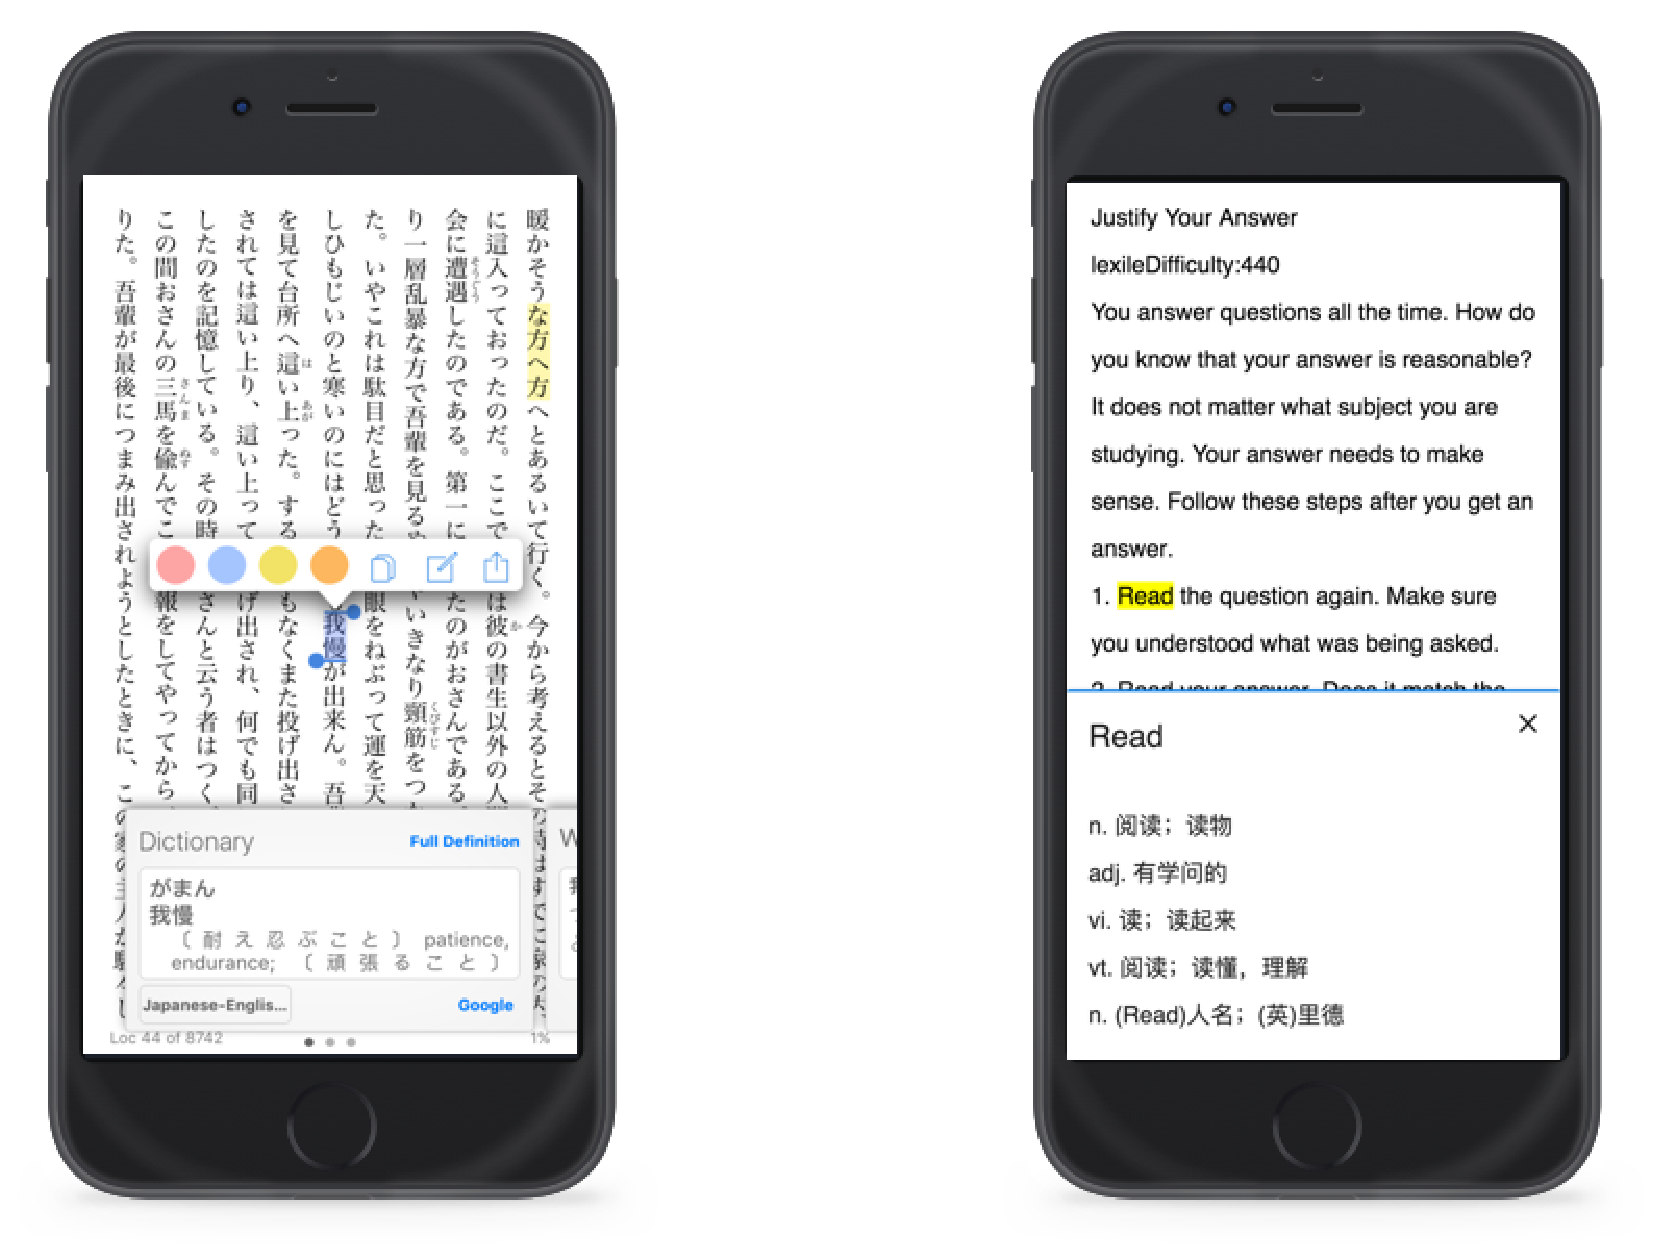
\includegraphics[width=120mm]{comparison_proposed_kindle.eps}
 \end{center}
 \caption{\label{figure:translation_module_vs_kindle} The proposed translation annotation module vs the translation annotation module in Kindle}
\end{figure}

\section{Relative difficulty vs weighted relative difficulty}

Carver first proposed the idea of relative difficulty in 1994 stating the difficulty of the reading isn't same for every learner, to more accurately measure the difficulty of the reading in correspondence to each learner, a measure of relative difficulty between one specific reading and one specific user is needed. Later on, in Carver's study, he conducted experiences on students and provided a formula for measuring the relative difficulty which is defined as the percentage of unknown words that a user has towards a specific reading. At the early stage of this study, only Carver's definition of relative difficulty is adopted as the based on the proposed recommendation system. However, in the data collection process, several problems were detected:
\begin{enumerate}
  \item First, unlike Carver did in his research where every user intentionally picked out all the unknown vocabulary. While using the Adaptive Learner, no all user will click on every unknown word, because sometimes knowing or not knowing a single vocabulary in the reading doesn't affect the overall understanding of the reading, or the unknown word could be simply omitted by the user due to careless or skip on sentences. Because all users have their own reading habits, and these habits closely connect to how they utilize the translation annotation module that the system provides. 
  \vspace{10pt}
  \item Second, human error exists while users are reading on the proposed system. Because there exist many actions that a user can perform on a web page such as scrolling, sometimes the user meant to perform another action, scroll to see the rest of the article, but a word was clicked the translation annotation module was triggered and recorded by the system. This happens particularly often when users are using the application on their smartphones. How to mitigate the effect of these mishandling on the result of relative difficulty has been an issue. 
  \vspace{10pt}
  \item Third, in Carver's definition of relative difficulty, every unknown word are weighted the same. In Carver's definition, all the words are weighted equally meaning that the unknown word “the” has exactly the same effect to user's language level profile as the word “apocalypse”. However, if a user doesn't know a very simple word, then it's very unlikely that he knows any word that is way harder than the unknown simple word. 
  \vspace{10pt}
\end{enumerate}

To mitigate the issues that were detected during the data collection process, a weighted relative difficulty is proposed. The proposed weighted relative difficulty uses frequency of the words as standard to apply a weight on every unknown word that user has clicked through the translation annotation module. By doing so, a word with a higher frequency such as ‘the' and ‘you' will weigh less to reduce the effect of misclicking on these words whereas a word with a lower frequency will weigh higher to increase its importance in calculating relative difficulty. Formula shows how Carver's relative difficulty is calculated while Formula shows how the proposed weighted relative difficulty is calculated. Both definitions are used later on to distinguish which measure is better suited for our method.

\section{A run-time estimator of relative difficulty}

The proposed system uses relative difficulty as the base measure to determine the distance between a reading and a user. Hence, it is critical for the system to be able to estimate readings' relative difficulty in terms of each user in order for the recommendation system to recommend articles to the users based upon these estimations. For finding the best estimator that can most accurately predict the relative difficulty of each reading in correspondence to each user, two types of estimation models were attempted. One is called the collaborative filtering which is a method used extensively in most of the online recommendation system, the other one is called linear regression method, which is chosen due to the continuous nature in the dataset.

\subsection{Collaborative Filtering}

\begin{figure}[tbp]
 \begin{center}
  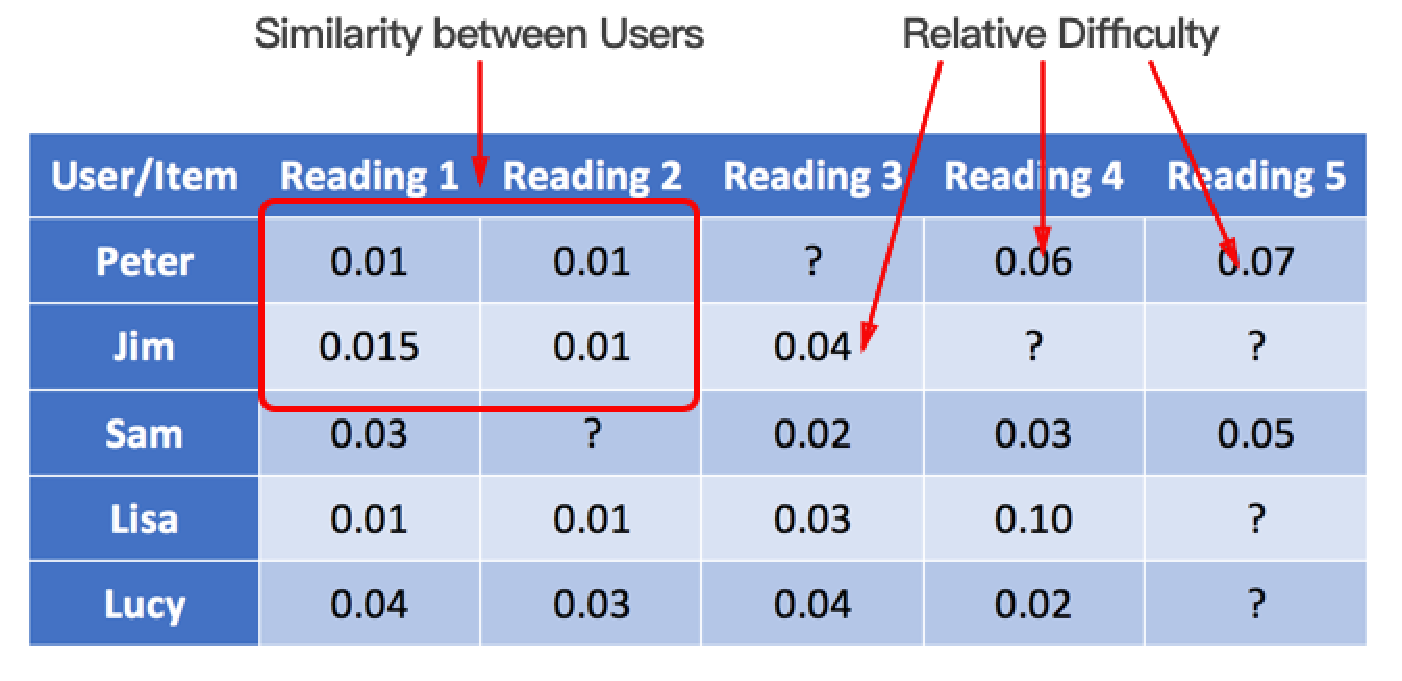
\includegraphics[width=100mm]{relative_difficulty_matrix.eps}
 \end{center}
 \caption{\label{figure:relative_difficulty_matrix} A recommedation matrix filled with the relative difficulty}
\end{figure}

Unlike the tradition recommendation system that recommends items based on user interest, the recommender in this study recommends items based on relative difficulty. To accomplish such tasks, our system first calculates the relative difficulty of each user towards each reading using the translation annotation module. More specifically, natural language processing is used to find all unique words in each reading. Then the number of unknown words was collected through the translation annotation module by counting how many unique words that a user has selected. Finally, the relative difficulty is calculated using Equation (\ref{eq:carver_relative_difficulty_1}), as it is defined by Carver.

\begin{equation}\label{eq:carver_relative_difficulty_1}
   Carver's \, Relative \, Difficulty = \frac{Number \, of \, unknown \, vocabulary}{Number. \, of \, total \, unique \,vocabulary \, in \, the \, reading}
\end{equation}

In this study, another weighted relative difficulty defined as shown in Equation (\ref{eq:weighted_relative_difficulty}) is also proposed to mitigate the issues detected as it was explained in the section Relative difficulty vs Weighted relative difficulty.

\begin{equation}\label{eq:weighted_relative_difficulty}
 Weighted \, Relative \, Difficulty = \frac{\sum_{k = 1}^{n} vocabulary \, frequency}{Number \, of \, total \, unique \,vocabulary \, in \, the \, reading}
\end{equation}

After obtaining all the relative difficulty of each user towards each reading, the recommendation matrix was constructed as shown in Figure~\ref{figure:relative_difficulty_matrix}. So the cell at column A and row W means the relative difficulty of item W to user A is 0.014. With the recommendation matrix constructed, we can now calculate the similarity user-wise and item-wise using cosine similarity as it is defined in Formula (\ref{eq:cosine_similarity}). 8 collaborative filtering based algorithms were used in this study to test and evaluate which algorithm will most accurately predict the relative difficulty of articles that user hasn't read given user's reading history. The 8 algorithms include SVD, Normal Predictor, SVDpp, KNNBasic, KNNBaseline, BaselienOnly, SlopeOne, KNNWithMeans, KNNWithZScore. 

\subsection{Linear Regression}

\begin{figure}[tbp]
 \begin{center}
  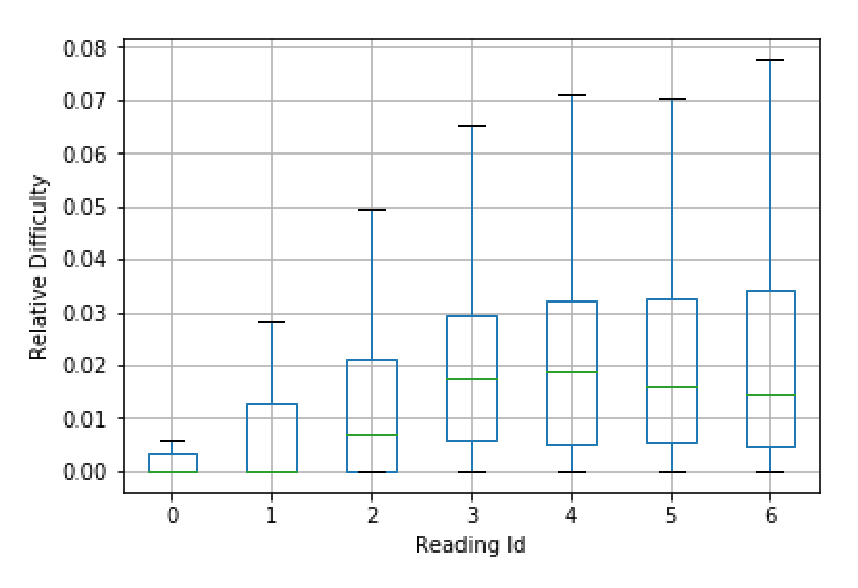
\includegraphics[width=100mm]{data_all_RD_rid.eps}
 \end{center}
 \caption{\label{figure:all_RD_rid} A box plot of user's relative difficulty distribution on of each reading}
\end{figure}

\begin{figure}[tbp]
 \begin{center}
  \includegraphics[width=120mm]{data_each_rd_vs_uid.eps}
 \end{center}
 \caption{\label{figure:each_rd_vs_uid} Plots of relative difficulty vs user's language level measured in user's total number of unknown clickings}
\end{figure}

\begin{figure}[tbp]
 \begin{center}
  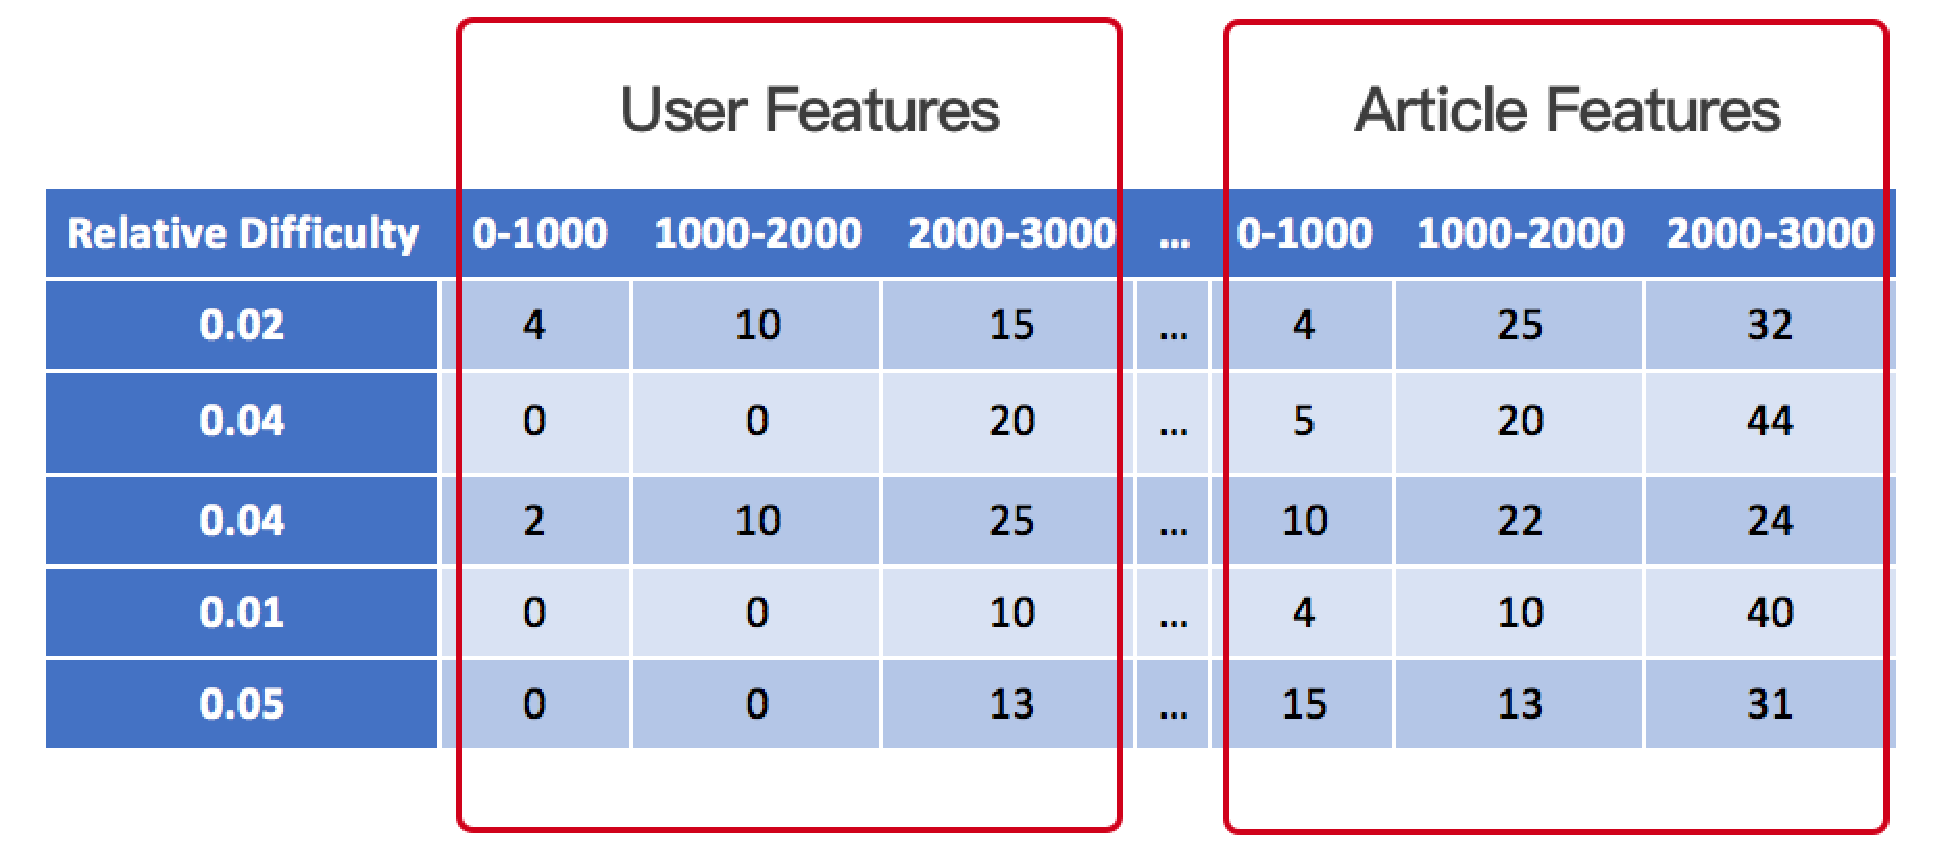
\includegraphics[width=100mm]{linear_features.eps}
 \end{center}
 \caption{\label{figure:linear_features} Features used in linear regression model: the user feature 0-1000 indicates the number of unknown clickings this user made in total that has a frequency between 0 and 1000, the article feature 0-1000 indicates the number of words that this articles contains with a frequency between 0 to 1000}
\end{figure}

Due to the dataset's regressive data nature, a simple linear regression model is also used in this study to compare with the traditional recommendation algorithms. Figure~\ref{figure:all_RD_rid} is a box plot where y-axis is the relative difficulty and x-aixs is the reading id. As it was stated before, the readings in the database are from easy to hard. Therefore, this box plot illustrates that there is a positive relationship between the relative difficulty and the reading difficulty level. It is reasonable to think, in general, the harder the general difficulty is, the higher the relative difficulty would be for each user. Of course, there will be outliers in the situations, such as, readings with specific terminologies in which people with knowledge of these words can easily understand, but people without knowing them can hardly understand. Because the relative difficulty is not only affected by the difficulty level of the readings, it is also affected by the language level of the users. The plots of each reading, where y-axis is the relative difficulty and x-axis is the user language level presented numerically as the measure of total amount of clickings that a user has made on all the readings, are also presented in Figure~\ref{each_rd_vs_uid}. There are 7 graphs in total in Figure~\ref{each_rd_vs_uid} where each graph presents the relationship between the total number of unknown clickings of the users and the relative difficulty. A positive relationship between the total number of unknown clickings of the user and the relative difficulty can be observed in all graphs, this relationship is particularly obvious in reading 4 and reading 5.

Data prepared for linear regression model is quite different from the data prepared for collaborative filtering. The linear regression model takes slightly different features as input. Instead of the recommendation matrix shown in Figure~\ref{figure:relative_difficulty_matrix}, the linear regression model takes both features from the articles and from the user forming a feature vector as shown in Figure~\ref{figure:linear_features}. For the linear regression model, the accumulated data is input as the user profile. This means that if a user has read 3 articles and the total amount of unknown clicking is 25. All 25 unknown clickings are used as user language level profile. All the unknown clickings are then classified into many groups based on their frequency. For example, the word “hello” has the frequency of 47.86 and it is placed into the group of frequency 0 - 1000. Each group is used as a feature for the user profile and the frequency range of the group is determined through running all combinations of possible groups from 1 to 100. In every combination, the linear regression model was constructed. 

\subsection{A recommendation system based on the run-time estimator of relative difficulty}

An accurate user profile is the key to good recommendations for the users \cite{Tan1998}. There are systems \cite{Klausmeier1977, Kuo2014} that require users to manually input their profiles, which places an extra burden on users. These kinds of manual work reduce users' interest in continuing using the application \cite{Tan1998}. Instead, systems that are capable of automatically constructing user profile through tracking users' interaction with the system are more preferable. Recent recommendation systems often track user's interaction action such as likes/dislikes, review, rating, and etc to form the user profiles. 

In personalized reading recommendations for the language learner, most of the systems \cite{Hwang2010, Kuo2014} are still in the stage of having users manually input their profiles through procedures such as pre-tests. In Hsu's research \cite{Hwang2010}, a pre-test and a questionnaire were given to evaluate the English reading ability and preferences of the students. In Kuo's research \cite{Kuo2014}, student's writing homework was selected as input to evaluate student's language level. Like the traditional recommendation systems, the use of pre-test will reduce user's interest in continuing user the application. Hence, either Kuo or Hus's system is applicable to large-scale user systems such as Newsela \cite{Newsela}, a platform for English learning through news reading.

In this study, we proposed a recommendation system that provides personalized reading recommendations based on the run-time estimator of the relative difficulty. The recommendation system takes the estimation of the relative difficulty of the readings and labels these values to next to each reading that is recommended to every user. The recommendation system was designed to recommend readings with lower relative difficulty to the users so that they can fully understand the content of the reading.

%%%%%%%%%%%%%%%%%%CHAPTER BREAK%%%%%%%%%%%%%%%%%%%%%%%%%%%%%%%%%%%%%%%%%%%%%%%%%%%%%%%%%%%%%%%%%%%%%%%%

\chapter{Dataset and Data Collection Process}

%%%%%%%%%%%%%%%%%TODO%%%%%%%%%%%%%%%%%%%%%%%
% \begin{figure}[tbp]
%  \begin{center}
%   
\includegraphics[width=80mm, height=80mm]{test.eps}
%  \end{center}
%  \caption{\label{figure:user_reading_time} The time that each user spent on each reading}
% \end{figure}

% \begin{table}[btp]
%  \caption{\label{table:user_reading_time} The average and median of time that each user spent on each reading}
%  \begin{center}
%   \begin{tabular}{ccc}
%    \hline
%    col1 & col2 & col3 \\
%    \hline
%    itema1 & itema2 & itema3 \\
%    itemb1 & itemb2 & itemb3 \\
%    itemc1 & itemc2 & itemc3 \\
%    \hline
%   \end{tabular} 
%  \end{center}
% \end{table}

As suggested in Chapter Method, the dataset that needed for the proposed method of work requires relative difficulty, which can be calculated through tracking user's unknown clickings on the articles. Because the weighted relative difficulty is later proposed, not only the total number of unknown words is required, but also the word itself needs also be recorded in the dataset. To be able to acquire such data from the users, the system needs to at least provide a translation annotation module and record all the interactions that users make with the system through the translation module.

Even though many applications such as Amazon Kindle \cite{Kindle} and Seed \cite{Seed} provide the translation annotation module in their applications. It doesn't necessarily indicate that they track the data that were required for testing the proposed method. After thorough research, no public datasets exist that provides the dataset, which is required for testing and evaluating the proposed system. We have contacted Amazon Kindle and Seeder to ask them if they have tracked the user unknown clickings in their application, and if so could they provide the data to us for research purpose. None of them replied. Therefore, we had no choice but to conduct the data collection process on our own. Later on, a one-year long data collection was carried out online. In March 2017, Adaptive Learner, the responsive website that was developed specifically for collecting the proper data from the users in order to verify the proposed method, was published. By March 2018, the total amount of users registered on the Adaptive Learner is 328. 

All the participants' native language is Chinese. Even though our application's translation annotation module supports English to Chinese and English to Japanese and a research question of whether the method will work the same for people with different native language was proposed at the beginning of the research, due to the time limitation, this question and functionality isn't verified in this thesis. The participants are mainly students from different grades. The invitation of participants is mainly through two means:
\begin{enumerate}
  \item Peer-to-peer, where I asked my friends to distribute the website and ask them and their friends to participate in the data collection;
  \item Working with several tutoring-centers, where I provided them with an online Toeic test practice website in exchange for having their students to join the data collection.
\end{enumerate}

In total three different tutoring centers have collaborated with us in data collection phase. One of them is located in Tokyo which is the one that we have received a lot of help from throughout this research. We would like to express our sincere appreciation to them in the Acknowledgement section. The final datasets can be found at \cite{dataset}. An example of a user's final data in JSON format is shown in Appendix A.

\section{Article data}

\begin{figure}[tbp]
 \begin{center}
  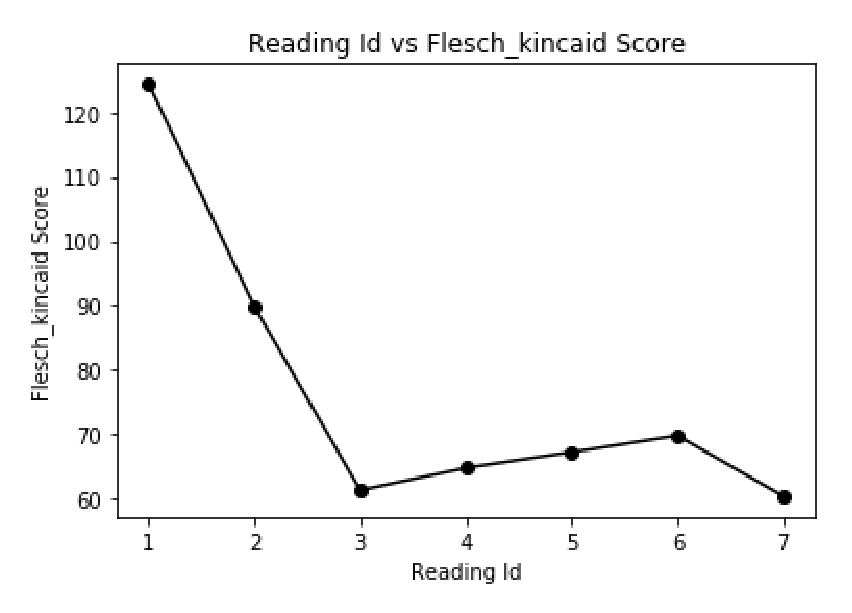
\includegraphics[width=100mm]{data_fk_rid.eps}
 \end{center}
 \caption{\label{figure:fk_rid} Reading readiablity calculated using Flesch-Kincaid Algorithm}
\end{figure}

\begin{figure}[tbp]
 \begin{center}
  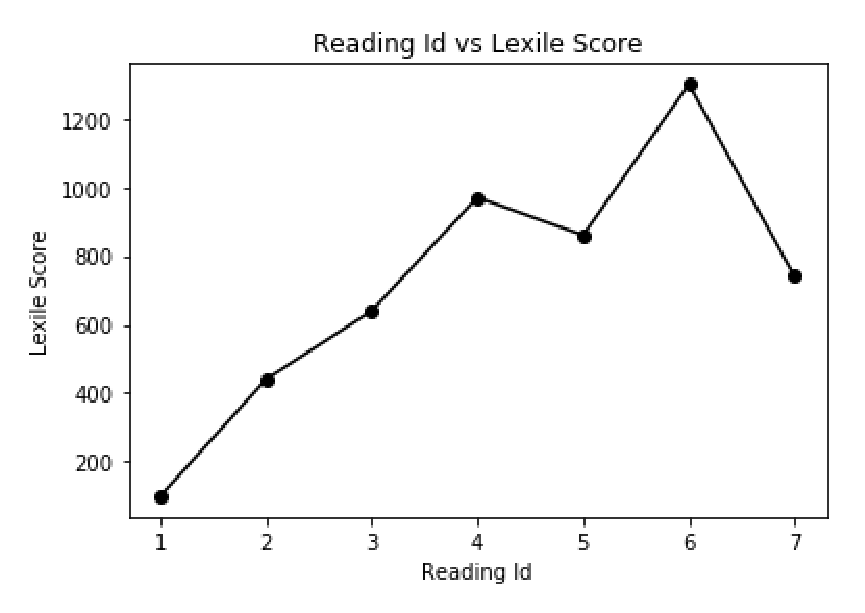
\includegraphics[width=100mm]{data_lexile_rid.eps}
 \end{center}
 \caption{\label{figure:lexile_rid} Reading readiablity calculated using Lexile Framework}
\end{figure}

All participants joined our research were required to read 7 different readings which are arranged from easy to hard. The article readability is determined based on both the Flesch-Kincaid measures \cite{Kincaid1975} and Lexile Score \cite{Lexile1996}. The Flesch-Kincaid scores of the readings are shown in Figure~\ref{figure:fk_rid}. The Lexile scores of the readings are shown in Figure~\ref{figure:lexile_rid}. The reading 1 through 3 has clear difference in difficulty, however, in reading 4 through 7, their difficulty is very close to each other. This variation between the distance of each reading in difficulty provides variation in data for evaluation purpose. All 7 readings are selected from the K12Reader, which is a popular educational reading material website \cite{K12Reader}. At the beginning of the research, there was the debate of whether more articles should be added to the database. Initially, 83 readings were imported to the article database to provide users with variation in content. And each user would still read seven articles but the articles provided to the users would be different, which may result in some users don't share anything in common meaning that two users haven't read the same article. After serious consideration, we decided to provide the same 7 readings for all users to generate more connections in data.

\section{User data collection}

\begin{figure}[tbp]
 \begin{center}
  \includegraphics[width=100mm]{data_collection_procedure.eps}
 \end{center}
 \caption{\label{figure:data_collection_procedure} User data collection procedure}
\end{figure}

The flowchart of the steps in the conducted data collection is shown in Figure~\ref{figure:data_collection_procedure}. These steps can be ordered as follow:

\subsection{Instruction for the experiment and user agreement}
\vspace{10pt}
When participants first visit the Adaptive Learner, there shows a thank you note and a short instruction for this data collection. By the end of the instruction, it shows a short user agreement stating that all users participate in this research agree to have the application record and track their data and agree to have the data to be used for research purpose. 

\subsection{User registration}
\vspace{10pt}
To be able to identify each user and add relative user profile information to each unique user, a simple user registration and login module are implemented. Many implementations were considered to simplify the signup process for each participant, such as record the IP address of every access to identify users or embed a cookie in the browser to identify each user. By the end, we decided to have users pick a unique nickname as their login to ease the user account registration process. This implementation is relatively easy and did work smoothly in a not so big user group. If users couldn't finish all the readings at once, they can always log back in using only the username they have picked to continue reading at where they have left off. Later on, to further reduce participants workload, a unique username is automatically generated for each user when they first visited the website, they can choose to edit it or just use it for registration.

\subsection{Collecting user's basic information}
\vspace{10pt}
After a simple registration, participants were asked to complete a short questionnaire about their background including education status, age, and etc. Users can choose not to answer most of the question, but one field is required called self-evaluation of language level. This field is proposed at the beginning of the research, for providing users with readings that closely match their language ability when no information has been collected about them. 

\subsection{Reading the articles}
\vspace{10pt}
After filling the short questionnaire, the readings are presented to each user one by one in order from the easier ones to the harder ones. During the reading process, the translation annotation module was provided to the users. Participants can press or select any unknown words or phrases, the translation of the words and phrases will appear at the bottom in their native language. During this process, every time that participants used the translation annotation module, the system will record it. Also, the system will record the start time and end time of each user reading each article to calculate how much time it takes each user to finish each article.

\subsection{Questionnaire after each reading}
\vspace{10pt}
All participants are asked to fill out a short questionnaire after each reading. If the participant did use the translation annotation module during the reading process for unknown word translation, the questionnaire would ask the user to pick out the words that they still remember the meaning of. Another question is how hard each user personally thinks the reading is according to their own current language level. The scale of this question is between 1 to 10, where 1 means that it is not hard at all, and 10 means it is way too difficult. Later on, we found that whether user remembers what they have translated using the translation annotation module isn't so relevant to the proposed method. These collected data weren't used in the proposed method.

\subsection{Reading data preprocessing}
\vspace{10pt}
In the proposed method, the readings are not imported directly as input to our data model. So it requires some preprocessing work before importing them into the data model. Because the proposed method adopted the idea of Carver's relative difficulty \cite{Carver1994}, it is important that we can calculate the relative difficulty from the data we collected. Carver states that one way of measuring relative difficulty is through the percentage of unknown words that a user has towards a specific reading. To calculate the percentage of unknown words, we need to obtain both the number of unknown words that a user has towards a reading, which can be obtained from the translation annotation module and the total number of unknown words in the article, which can be obtained through reading data preprocessing. In this step, the NLTK package was used to find all the unique words in a reading. The NLTK package provides a function to identify words in singular form and plural form. In regular string manipulation, “animal” and “animals” are treated as two different words. By using the NLTK package, it is possible to identify words in its singular form and plural form as the same word so that an accurate total number of words can be found.

\section{User data validation}
User data validation occurs after user finished reading the materials that we provided. If a user didn't finish the entire data collection process meaning that this user didn't finish reading all the articles, this user's data will be treated as invalid data and excluded from the final datasets. Since the amount of time that each user reads each reading is recorded during the data collection, if a user took extra long or extra less time during the data collection, this abnormal behavior will be detected and the user data will be treated as invalid. These types of users' data were excluded from the final datasets. After user data validation, there remain 239 users whose data are verified for the research. These 239 users' data are entered into the final datasets and being used for training and validating the data model in the evaluation section.

%%%%%%%%%%%%%%%%%%CHAPTER BREAK%%%%%%%%%%%%%%%%%%%%%%%%%%%%%%%%%%%%%%%%%%%%%%%%%%%%%%%%%%%%%%%%%%%%%%%%
\chapter{Results and System Evaluation}

\section{Summary of the users' basic information}

\begin{figure}[tbp]
 \begin{center}
  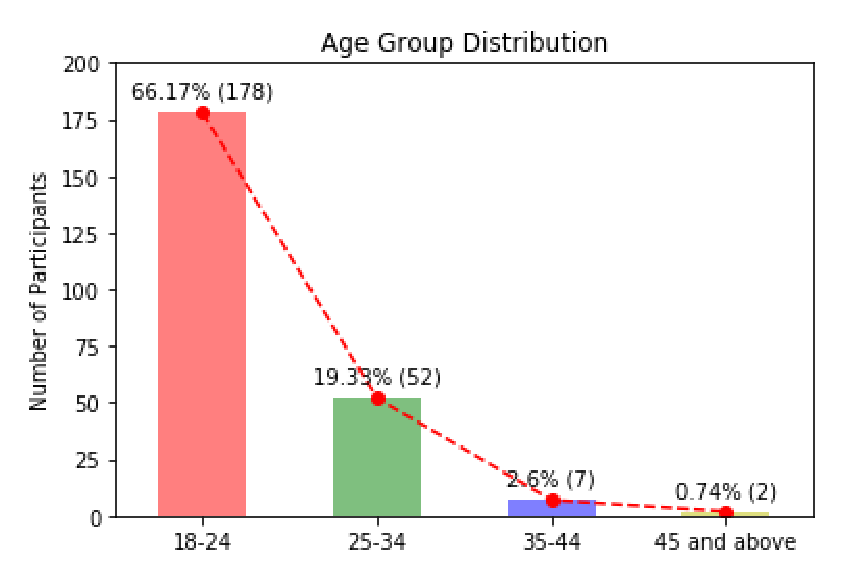
\includegraphics[width=100mm]{age_distribution.eps}
 \end{center}
 \caption{\label{figure:age_distribution} Age distribution of the participants}
\end{figure}

\begin{figure}[tbp]
 \begin{center}
  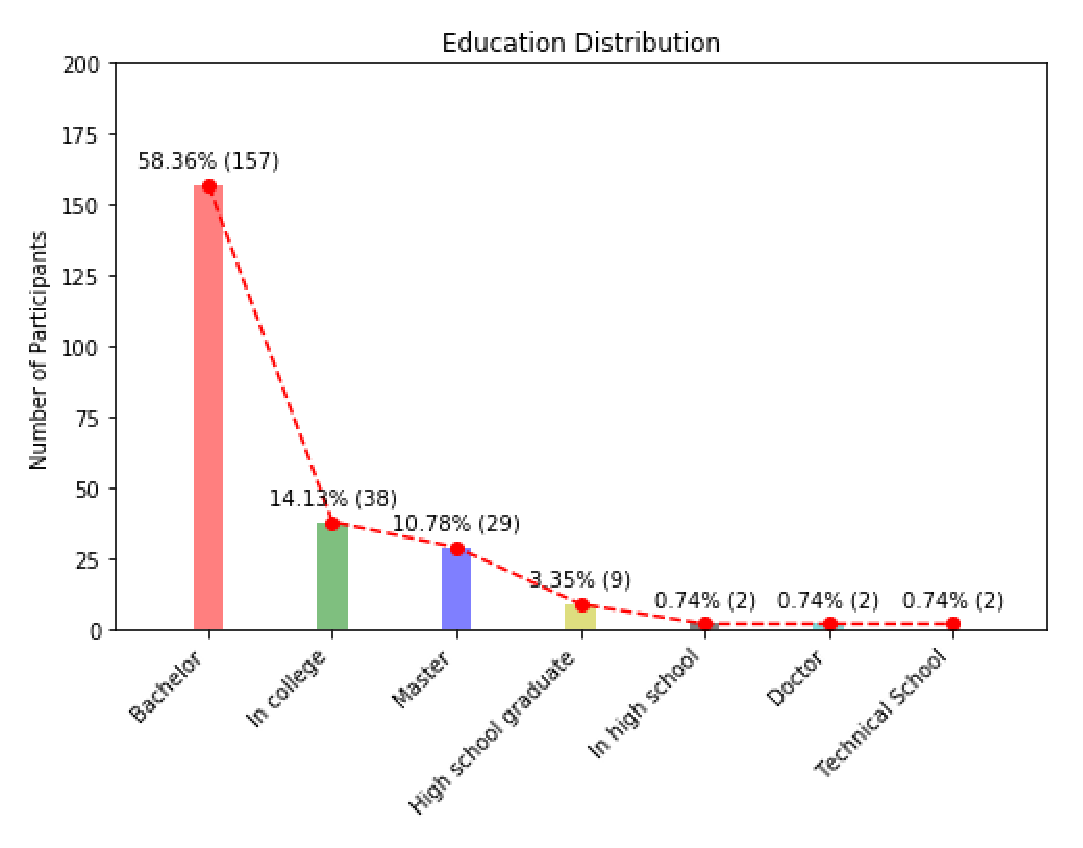
\includegraphics[width=100mm]{education_distribution.eps}
 \end{center}
 \caption{\label{figure:education_distribution} Education distribution of the participants}
\end{figure}

The total amount of users participated in this research is 328, in which 269 users' data passed through the data validation and added to our final datasets. The 328 users are all from China, which can be easily determined through the native language that they have picked while using the translation annotation module that the system provides. The age distribution of the participants is as shown in Figure~\ref{figure:age_distribution}. Most of the participants are in the age of between 18 to 34 due to the reason that all the participants are invited through peer-to-peer who are all in the similar age range as me. The education distribution of the participants is shown in Figure~\ref{figure:education_distribution}. 157 out of 269 users have obtained their bachelor degree and 29 out of 269 participants are graduated as masters. 

\section{Demonstration of similarity in users' relative difficulty}

\begin{figure}[tbp]
 \begin{center}
  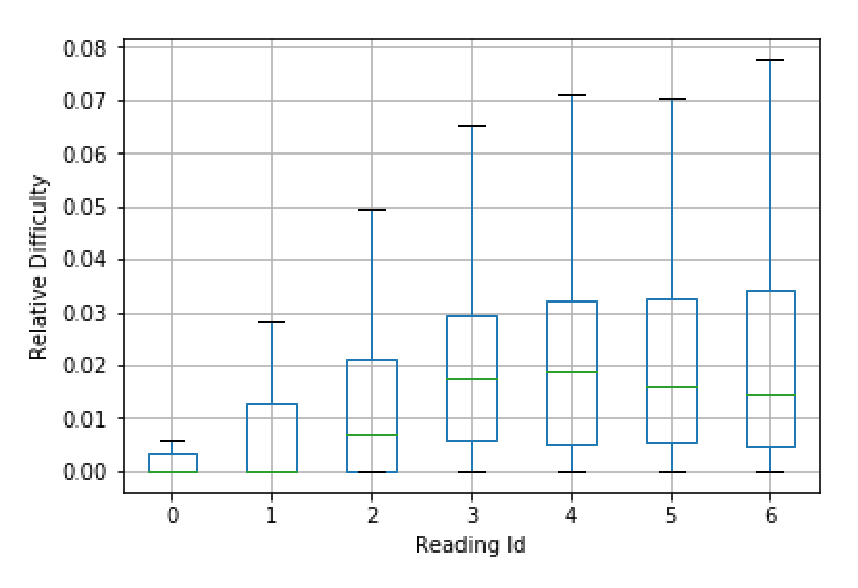
\includegraphics[width=100mm]{data_all_RD_rid.eps}
 \end{center}
 \caption{\label{figure:all_RD_rid} The relative difficulty vs reading readability}
\end{figure}

There are in total of 7 readings in our reading database, and each test subjects are required to read through all of them. The general difficulty of the reading increases from reading 1 to reading 7. Figure~\ref{figure:all_RD_rid} shows the distribution of relative difficulty for each user towards each reading. It is illustrated that on average the higher the reading difficulty is, the higher the relative difficulty for each user gets. The variation in users' relative difficulty of the same reading demonstrates the theory that the relative difficulty of the reading is different for each user. If we look at the relative difficult distribution of reading 6, the highest relative difficulty for a user is close to 0.08, while the lowest relative difficulty is 0. And the majority of the relative difficulty of reading 6 lies in between 0.005 to 0.035, which is a relatively big range. 

\begin{figure}[tbp]
 \begin{center}
  \includegraphics[width=120mm]{user_RD_similarity.eps}
 \end{center}
 \caption{\label{figure:user_RD_similarity} Plots of every article's relative difficulty for all users }
\end{figure}

Collaborative Filtering requires there to be similarities between users in order to predict the unknown information from a collaboration of other user's existing data. So it is critical to demonstrate that there exist similarities in users' clicking behavior, which indicates that there are also similarities in users' relative difficulty. Figure~\ref{figure:user_RD_similarity} shows graphs of each user's relative difficulty for each reading. The x-axis stands for each user's id whereas the y-axis shows the value of relative difficulty. All graphs in Figure~\ref{figure:user_RD_similarity} appears to be in a shape of stairs. Each step of the stair indicates a group of users who share the same relative difficulty for a specific article. For instance, 94 users' relative difficulty on reading 3 is 0; 62 users' relative difficulty on reading 3 is 0.01. In our datasets, we can split users into 14 groups based on each user's relative difficulty. The similar trend can also be found in the rest of the articles which are shown in Figure. Because there exist similar users in our datasets, collaborative filtering methods should be a worthwhile data modal to attempt for predicting the relative difficulty of each user towards each reading. 

\section{Estimator evaluation}

\begin{figure}[tbp]
 \begin{center}
  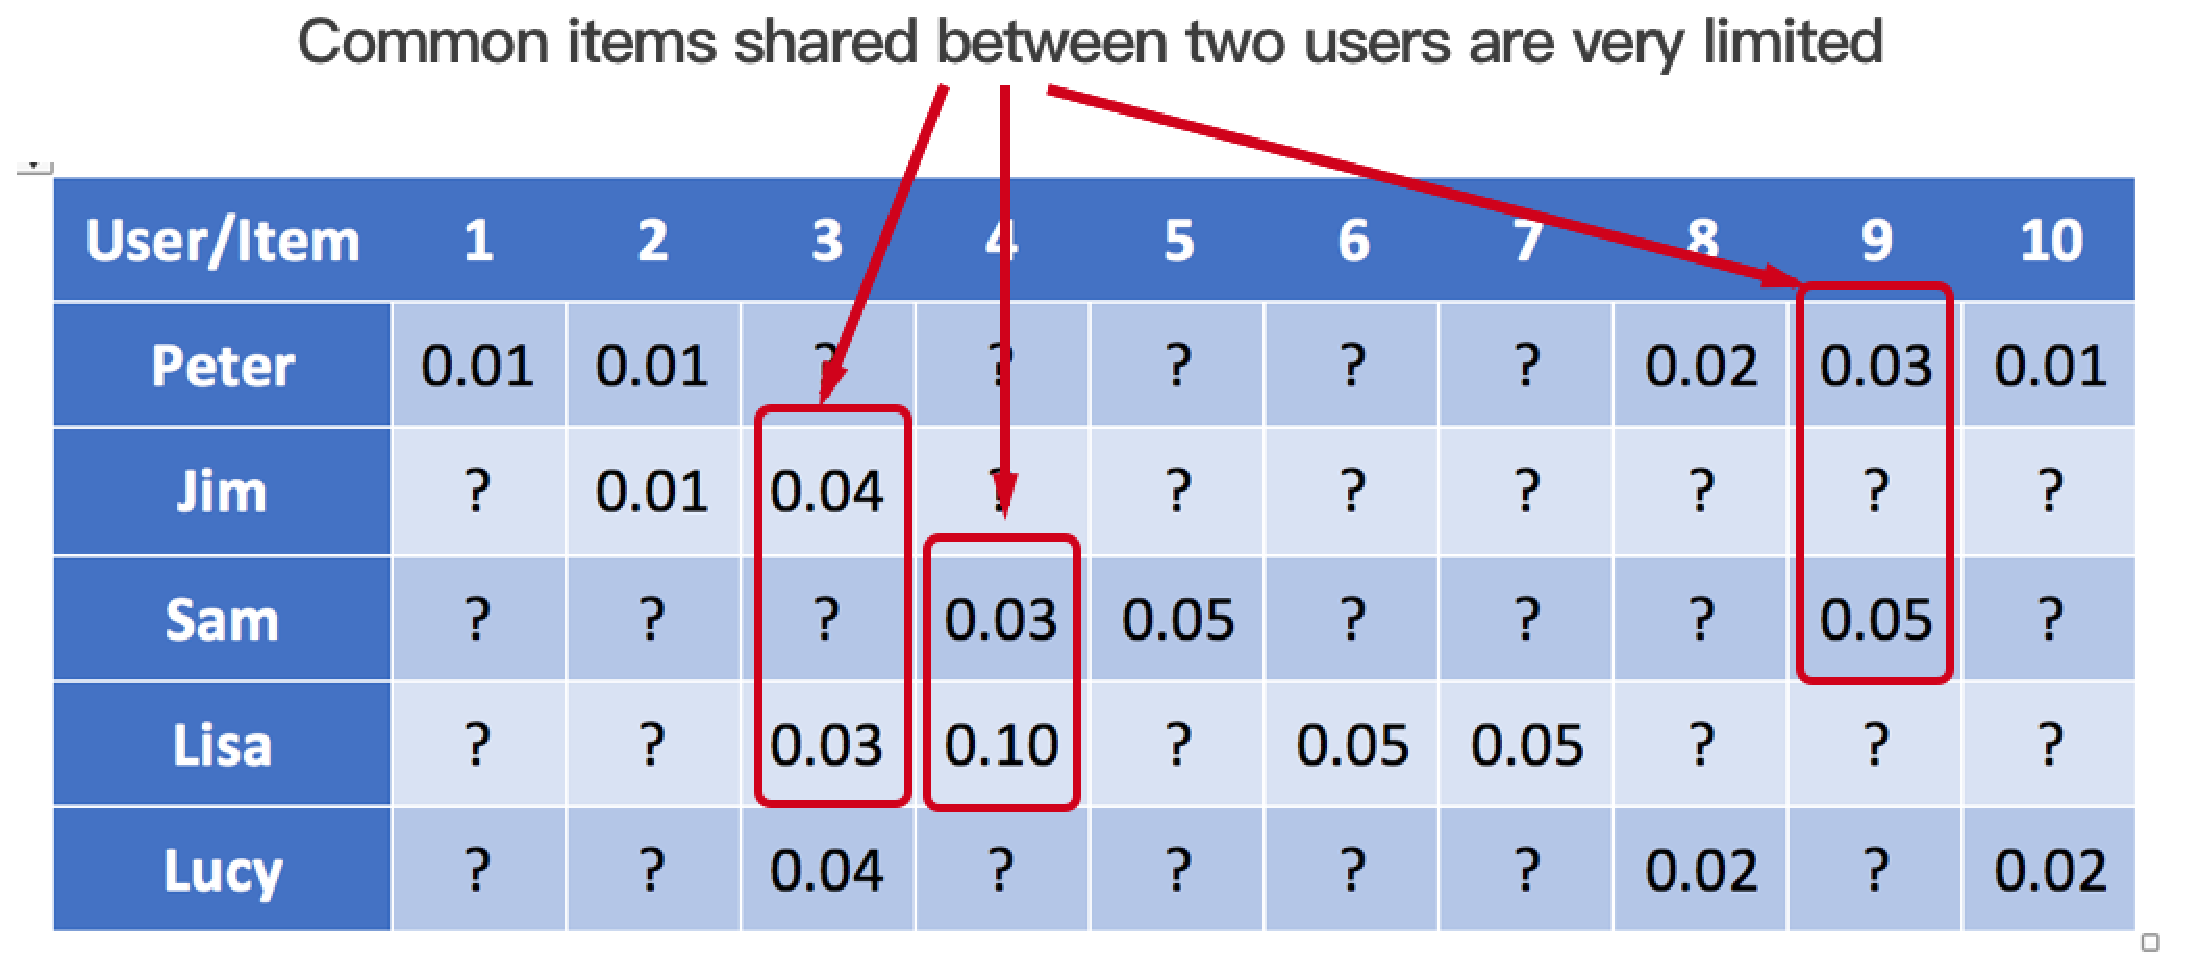
\includegraphics[width=100mm]{matrix_sparse.eps}
 \end{center}
 \caption{\label{figure:matrix_sparse} A typical sparsed recommendation matrix}
\end{figure}

\begin{figure}[tbp]
 \begin{center}
  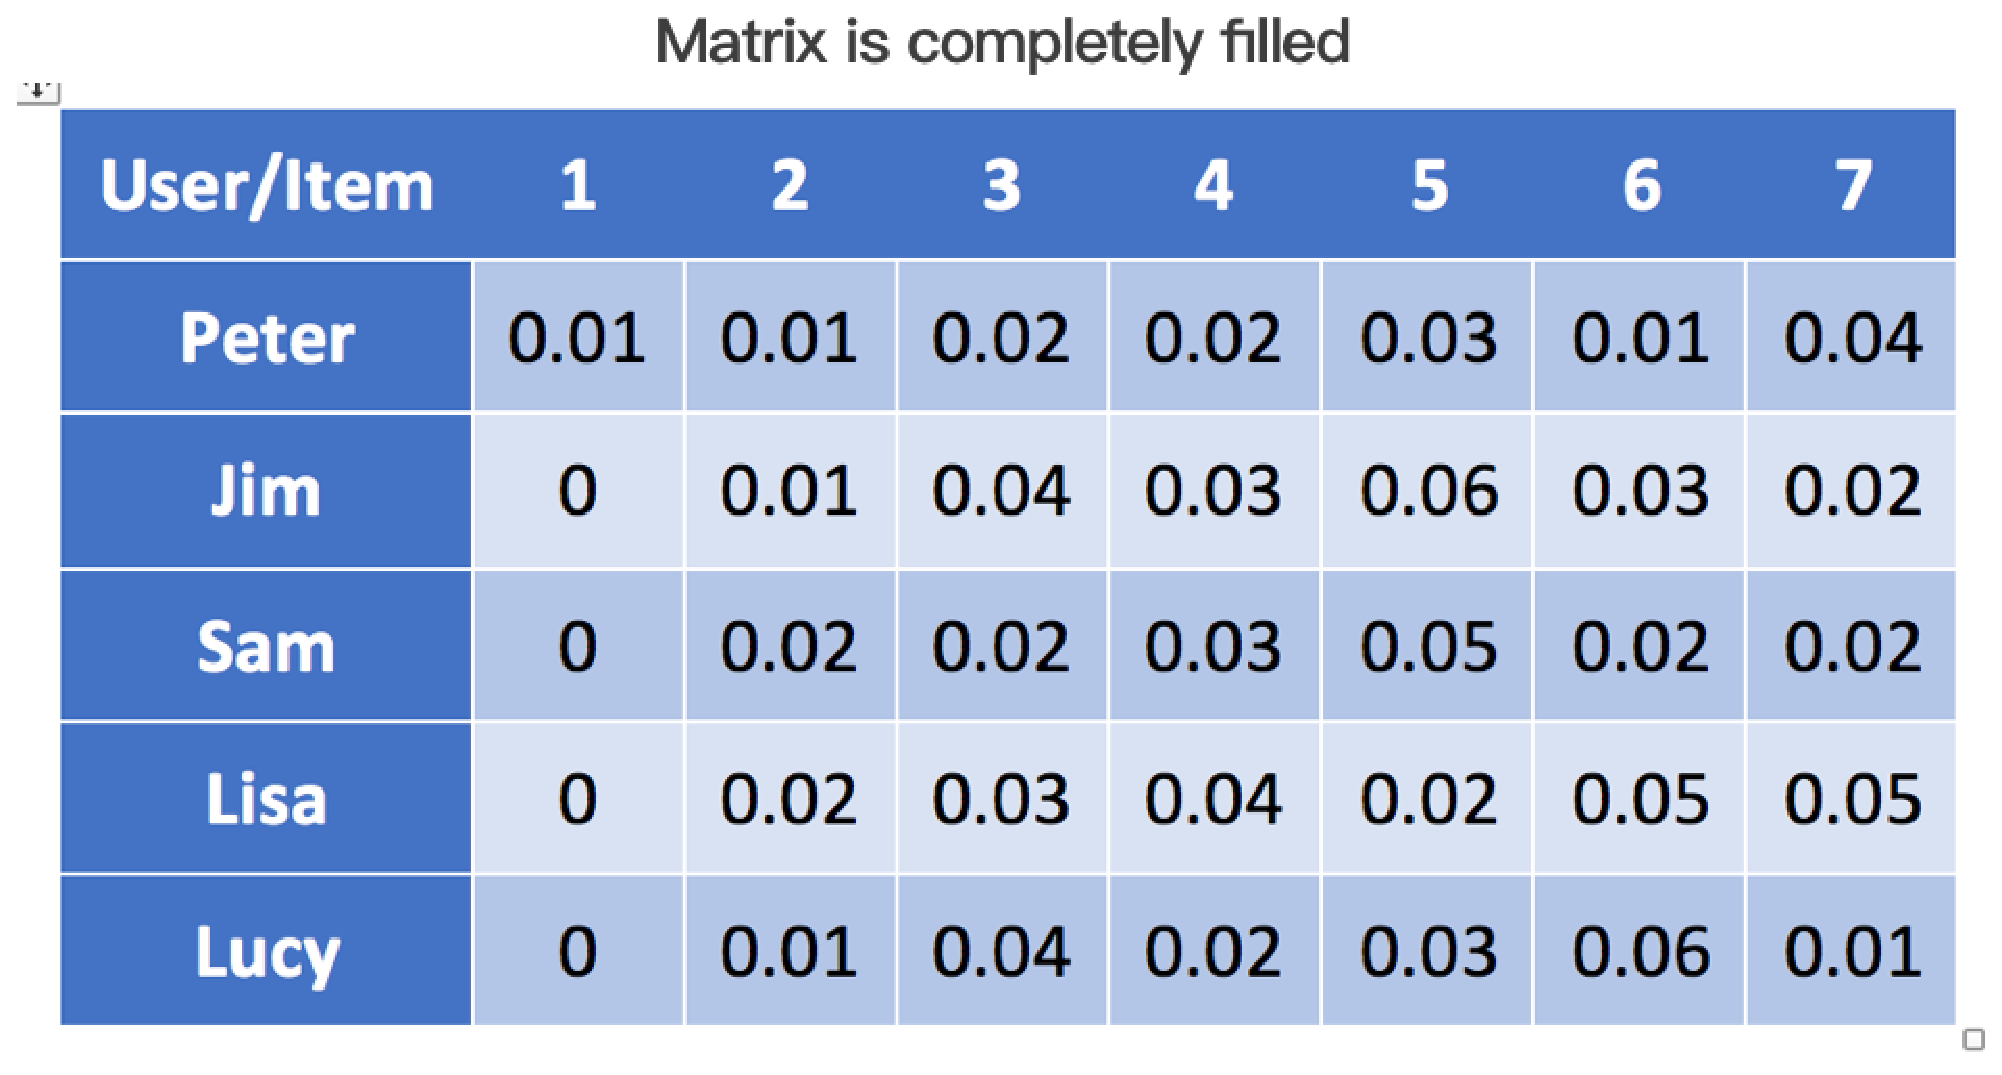
\includegraphics[width=100mm]{matrix_full.eps}
 \end{center}
 \caption{\label{figure:matrix_full} The recommedation matrix in this study}
\end{figure}

Scikit-learn and pandas python package is used extensively in the estimator evaluation. After data preprocessing, the obtained dataset is filtered and only the data needed for the recommendation matrix are used, which are user id, reading id, and the corresponding relative difficulty. After datasets are prepared into the right format for data model training purpose, nine popular algorithms including SVD, Normal Predictor, SVDpp, KNNBasic, KNNBaseline, BaselienOnly, SlopeOne, KNNWithMeans, KNNWithZScore are selected as data models for our estimator. To find out which existing algorithm can most accurately estimate the relative difficulty using the collected dataset, cross-validation was adopted in this study. The cross-validation is a model validation technique for evaluating how the results of a data model will generalize to an independent data set. There exist many types of cross-validation method. The one that was picked for evaluation is called k-fold cross-validation. In this validation method, the original data sample is randomly split into k equally partitioned subsamples. From the k subsamples, one sample is picked as the validation data for the testing purpose, and the rest k - 1 subsamples are used as training data. The cross-validation was then repeated k times, each time one of the randomly partitioned subsamples is used as test data while the other k - 1 subsample are used as training data. The advantage of this validation method is that all the data are used both as testing and training. 

\subsection{How accurate is the proposed estimator at predicting relative difficulty?}

\begin{equation}\label{eq:rmse}
   RMSE = \sqrt{\frac{1}{n}\Sigma_{i=1}^{n}{\Big(\frac{d_i -f_i}{\sigma_i}\Big)^2}}
\end{equation}

At each repetition of the cross-validation, the RMSE (root mean squared error) is calculated as the metrics for measuring the accuracy of all the data models. Equation (\ref{eq:rmse}) shows how RMSE is calculated. The average of the RMSE calculated at each repetition is used as the final RMSE for the data models. The RMSE is a very commonly used measurement of the difference between the predicted value by an estimator and the true value. Formula shows how the RMSE is calculated. Because the RMSE is a squared value, it is always non-negative. An RMSE of 0, which will never be achieved in practice, indicates a perfect data model that predicts all the data correctly. In general, a lower RMSE indicates better fitness of the data model. However, lower RMSE doesn't necessarily indicate a better recommendation.

\begin{table}[btp]
 \caption{\label{table:rmse_cf_algo} The RMSE for all the collaborative filtering algorithms}
 \begin{center}
  \begin{tabular}{ccc}
   \hline
   & Algorithm & RMSE (Root mean square error) \\
   \hline
   1 & KNNWithZScore & 0.0157 \\
   2 & KNNWithMeans & 0.0158 \\
   3 & SlopeOne & 0.0171 \\
   4 & KNNBaseline & 0.0178 \\
   5 & BaselineOnly & 0.0180 \\
   6 & KNNBasic & 0.0188 \\
   7 & SVDpp & 0.0236 \\
   8 & NormalPredictor & 0.0266 \\
   9 & SVD & 0.0459 \\
   \hline
  \end{tabular} 
 \end{center}
\end{table}

The cross-validation along with RMSE calculation was performed on every popular algorithm that was listed above. The number of folds for cross-validation was set to 10. The RMSE of each algorithm is listed in Table~\ref{table:rmse_cf_algo}. As indicated in the Table~\ref{table:rmse_cf_algo}, KNNWithZScore data model outperforms the rest with an RMSE of 0.0157 while the SVD algorithm performed worst with an RMSE of 0.0443. The famous SVD \cite{Salakhutdinov2007} algorithm was popularized during the Netflix Prize in which Simon Funk used it to won the prize. However, SVD algorithm performed worst in the collected dataset was very surprising. The possible reason is that most of the recommendation matrix used in regular recommendation models are very sparse meaning that a lot of the users only watched movie A, B, C while the reading C, D, E haven't been watched. These kinds of recommendation matrix are shown in Figure~\ref{figure:matrix_sparse}. SVD based algorithms are very strong at finding out the latent factors between two users with no movies that both of them have watched and rated. However, in dataset collected in this study, every participant are required to read all the readings provided meaning that the recommendation matrix formed in this study has 0\% sparsity as shown in Figure~\ref{figure:matrix_full}. This fully filled recommendation matrix is suspected to be the cause of the low performance of the SVD based algorithms. 

\subsection{Can proposed system be able to adapt to user's profile change?}

\begin{table}[btp]
 \caption{\label{table:rmse_cf_algo_leave_p_out} The RMSE of KNNWithZScore using leave-p-out cross validation}
 \begin{center}
  \begin{tabular}{ccc}
   \hline
   p & RMSE  \\
   \hline
   Leave 1 out & 0.0162 \\
   Leave 2 out & 0.0164 \\
   Leave 3 out & 0.0197 \\
   Leave 4 out & 0.0218 \\
   Leave 5 out & 0.0235 \\
   Leave 6 out & 0.0212 \\
   \hline
  \end{tabular} 
 \end{center}
\end{table}

Another question to answer is that how many articles that user should read so that data model can give a relatively good recommendation. To answer this question, another cross-validation method called leave-p-out cross-validation is used. Leave-p-out cross-validation is designed to use p observations as the validation set and the remaining observations as the training set. While using it in the collected dataset, p set to 1 meaning that one reading is used as validation set while the other 6 is used as the training set; p set to 6 meaning that training the model with one reading to predict the relative difficulty of the other 6. The result of the leave-p-out cross-validation is shown in Table~\ref{table:rmse_cf_algo_leave_p_out}. According to the Table~\ref{table:rmse_cf_algo_leave_p_out}, it is indicated that use six articles as training data to predict the relative difficulty of the remaining one has clearly the best performance. In general, the more the user reads in the system, the higher the accuracy the estimator gets. But even with one reading in the user profile, the system still has the ability to estimate. The decreasing trend in RMSE when more user profile data are added to the data model illustrates that the estimator does have the ability to adapt to the change in the user profile.

\subsection{Evaluation of the linear regression model}

The relative difficulty was also estimated using a linear regression model due to the continuous nature of the data. In the linear regression model, the frequency of the words in the reading are used as features for the readings, and the frequency of the words that users have clicked on are used as the features for the users. By using the features of both user and reading, the linear regression model was used to estimate the relative difficulty of a user with certain language skill towards a reading with certain readability. 

The same cross-validation method is used for testing the linear regression model. Surprisingly, the linear regression model was capable of achieving an RMSE of 0.0120, which outperforms all tested recommendation model. The coefficient of determination \cite{Glantz1990}, which is also called r-squared, is also used as an evaluation method for the linear regression. The coefficient of determination is a value between 0 to 1 that measures how well-observed outcomes are replicated by the model using the proportion of total variation of outcomes explained by the model. The result of the coefficient of determination and RMSE of both linear regression model and the best recommendation model can be found in Table~\ref{table:r2_linear_vs_cf}. We can see that both coefficient of determination and RMSE indicates that linear regression estimator is better at estimating users' relative difficulty in this dataset. 

\begin{table}[btp]
 \caption{\label{table:r2_linear_vs_cf} The coefficient of determination of the linear regression model and the best collaborative filtering model}
 \begin{center}
  \begin{tabular}{ccc}
   \hline
   Data Model & Coefficient of Determination & RMSE \\
   \hline
   Linear Regression & 0.539 & 0.0120 \\
   KNNWithZScore & 0.144 & 0.0157 \\
   \hline
  \end{tabular} 
 \end{center}
\end{table}

\section{Evaluation of the recommedation system}

\subsubsection{How good is the proposed recommendation system?}
\vspace{10pt}
Even though both collaborative filtering and linear regression models appear to be able to estimate the relative difficulty defined by Carver, the definition of relative difficulty by Carver is only one way of defining the distance between a user and a reading. A good prediction of the relative difficulty defined by Carver doesn't represent an accurate actual distance between a user and a reading. To truly evaluate the performance of our system at distinguishing the distance between a different user and a different reading, 10 test subjects were recruited. Each user was invited to read the first 5 articles which are used for constructing the user profile and rank the last two articles based on the difficulty of the artile in his/her own perspective. For example, if user A believe reading 6 is harder than reading 7 for him/her, then he/she can rate select reading 6 as the harder one between the two readings. The proposed system will also pick the harder readings based on the relative difficulty that the estimator estimates. All the data model evaluated in this study were tested for this experiment.

As it was mentioned above, the relative difficulty defined by Carver is merely one way of defining the distance between a user and an article. When Carver defined it during his research in the 1980s, he did it through participants intentionally circling out all the unknown words in the reading. In our system, participants can use the translation annotation module when they ran into unknown words. But they can also decide to ignore an unknown word and continue reading the article or click on a known word by accident or purposely checking out the functionality. It is very difficult to know whether a click made is equivalent to an unknown vocabulary. To mitigate these issues, a weighted relative difficulty is proposed in this study. A weighted relative difficulty is an idea based on Carver's research. In Carver's definition, each unknown words weighted the same as shown in Formula~\ref{eq:carver_relative_difficulty}. However, in the proposed system, each click can mean many things, such as misclick, system malfunction, or human error. We adopted the frequency of the vocabulary as the weight of each click. By doing so, a high-frequency word will weight less, such as misclick on common words such as “the” or “an”, while a low-frequency word will weight more to emphasize on this action's importance. The weighted relative difficulty is calculated through Formula (\ref{eq:weighted_relative_difficulty}). 

Same cross-validation method and estimators were performed using the new datasets where the weighted relative difficulty replaced the relative difficulty defined by Carver. Because the definition of the metrics changed, the comparison between the evaluation metrics such as RMSE or coefficient of determination is quite meaningless. Hence, only the percentage of the correct ranking estimation is compared. The percentage indicates the number of users' rankings matches exactly as the model estimated over the total number of users' rankings. Table~\ref{table:accuracy_ranking_linear_vs_cf} shows the best ranking results among all the data models. It can be easily recognized that the estimator using the weighted relative difficulty outperformed the estimator using Carver's relative difficulty.

\begin{table}[btp]
 \caption{\label{table:accuracy_ranking_linear_vs_cf} The accuracy of ranking the articles using the linear regression model, Collaborative Filtering with Carver's Relative Difficulty, and Collaborative Filtering with the Weighted Relative Difficulty}
 \begin{center}
  \begin{tabular}{ccc}
   \hline
   Algorithm & Correctness \\
   \hline
   Linear Regression & 50\% \\
   Carver's Relative Difficulty KNNBaseline & 80\% \\
   Weigthed Relative Difficulty KNNBaseline & 90\% \\
   \hline
  \end{tabular} 
 \end{center}
\end{table}
